\chapter{Statique des robots manipulateurs}
\label{sec:static}

%Chapitre en construction!

\section{Introduction}

Ce chapitre présente des méthodes pour déterminer les relations entre les divers forces agissant sur un robot manipulateur lorsque le système est à l'équilibre. La matrice jacobienne $J$, la même matrice de la relation de cinématique différentielle de l'équation \ref{eq:diffkinrel}, permet de transformer une force cartésienne $\col{f}_E$, que l'effecteur du robot applique sur l'environnement, en couples (ou force pour un joint prismatique) équivalents $\col{\tau}$ dans le domaine des joints:
%%%%%%%%%%%%%%%%%%%%%%%%%%%%%%%%%%%%%%%%%%%%%%%%%%%%%%%%%%%%%%
\begin{align}
\col{\tau} &= J\left( \, \col{q} \, \right)^T \, \col{f}_E
\label{eq:static1}
\end{align}
%%%%%%%%%%%%%%%%%%%%%%%%%%%%%%%%%%%%%%%%%%%%%%%%%%%%%%%%%%%%%%
Cette relation permet de calculer les liens entre les forces externes et les forces produites par les actionneurs sans avoir à déterminer toutes les forces internes du systèmes, ce qui particulièrement utile pour les robots manipulateurs et sera exploité par les méthodes de ce chapitre. 
%%%%%%%%%%%%%%%%%%%%%%%%%%%%%%%%
\begin{figure}[H]
	\centering
		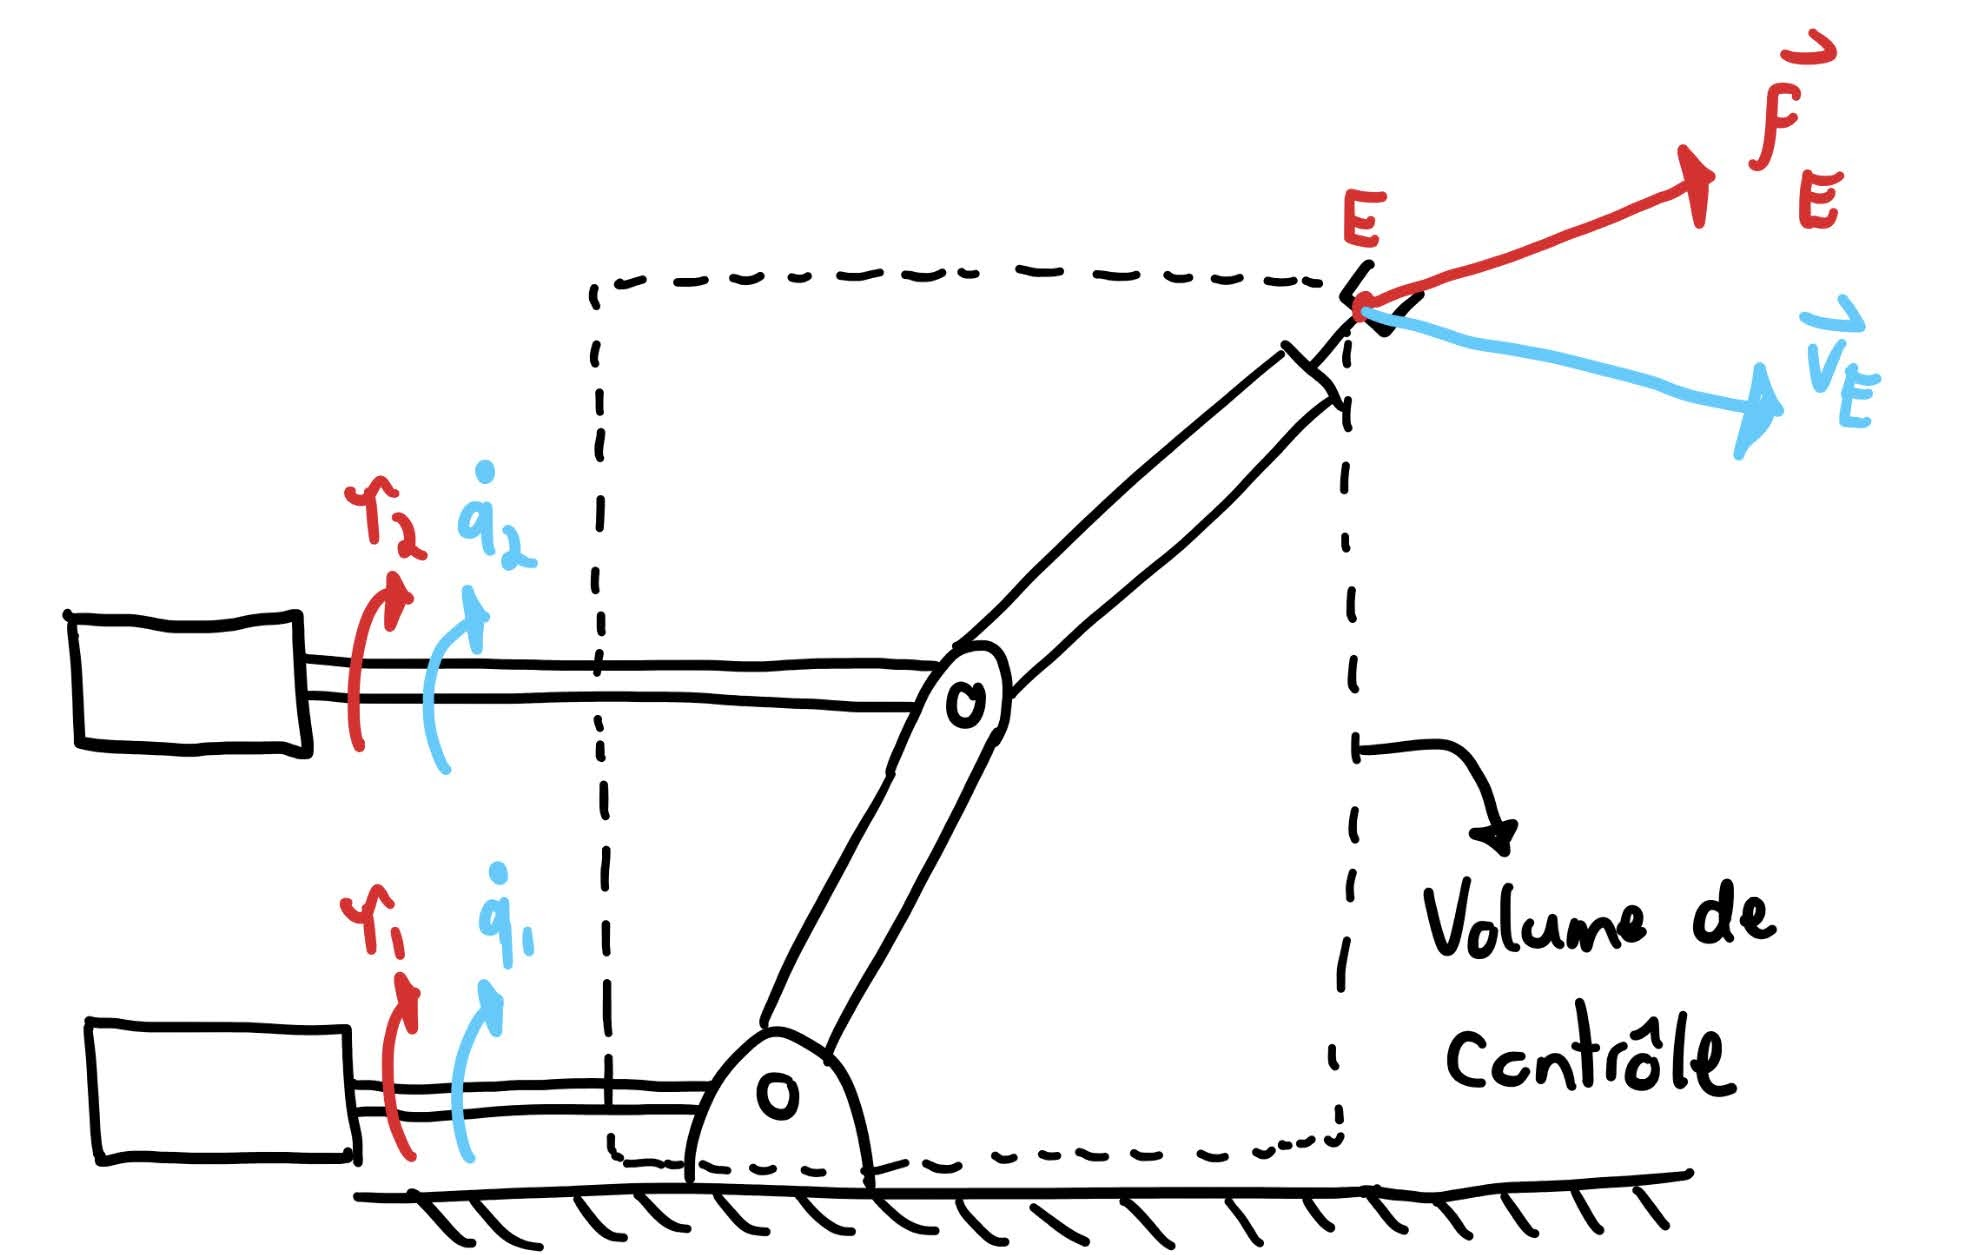
\includegraphics[width=0.55\textwidth]{fig/controlvolume.jpg}
	\caption{Bilan de puissance mécanique pour un robot manipulateur}
	\label{fig:controlvolume}
\end{figure}
%%%%%%%%%%%%%%%%%%%%%%%%%%%%%%%%

\video{Statique des robots manipulateurs}{https://youtu.be/klAfYgPYi0k}

\section{Les vecteurs forces}
\label{sec:force}

Une force est une quantité vectorielle avec une amplitude et une direction. Comme pour les notions de cinématique, nous utiliserons une notation qui distingue le vecteur-géométrique $\Vec{f}$ et le vecteur-colonne de composantes $\col{f}^a$ dans une base $a$. De plus, une force appliquée sur un corps $C$ à un point $A$ sera notée: 
%%%%%%%%%%%%%%%%
\begin{align}
\vec{f}_{C_A}
\end{align}
%%%%%%%%%%%%%%%%
Le principe d'action/réaction indique que si une force est appliquée sur un corps $C1$ il y a nécessairement une réaction égale et opposée sur un corps $C2$. Une force agissant sur un corps $C1$ par un corps $C2$ sera notée:
%%%%%%%%%%%%%%%%
\begin{align}
\vec{f}_{C1/C2}
\end{align}
%%%%%%%%%%%%%%%
et le principe d'action/réaction nous donne donc la propriété suivante:
%%%%%%%%%%%%%%%%
\begin{align}
\vec{f}_{C1/C2} = - \vec{f}_{C2/C1}
\end{align}
%%%%%%%%%%%%%%%
Cette notation sera utilisée lorsqu'il est question de forces d'interactions entre deux corps car le signe source de confusion lorsqu'on ne distingue pas la force appliquée \textit{sur} à la force appliqué \textit{par} un objet.

Dans ce chapitre, nous définirons un vecteur $\vec{f}_{R_E}$ comme un force appliquée sur le robot à un point $E$ (typiquement l'effecteur) par l'environnement, et $\vec{f}_{E}$ comme son inverse, i.e. la force que le robot applique sur l'environnement:
%%%%%%%%%%%%%%%%
\begin{align}
\vec{f}_{R_E} &=\vec{f}_{Robot/Environment} \\
\vec{f}_{E}   &=\vec{f}_{Environment/Robot} = -\vec{f}_{R_E}
\label{eq:contactforcenotation}
\end{align}
%%%%%%%%%%%%%%%

%%%%%%%%%%%%%%%%%%%%%%%%%%%%%%%%
\begin{figure}[H]
	\centering
		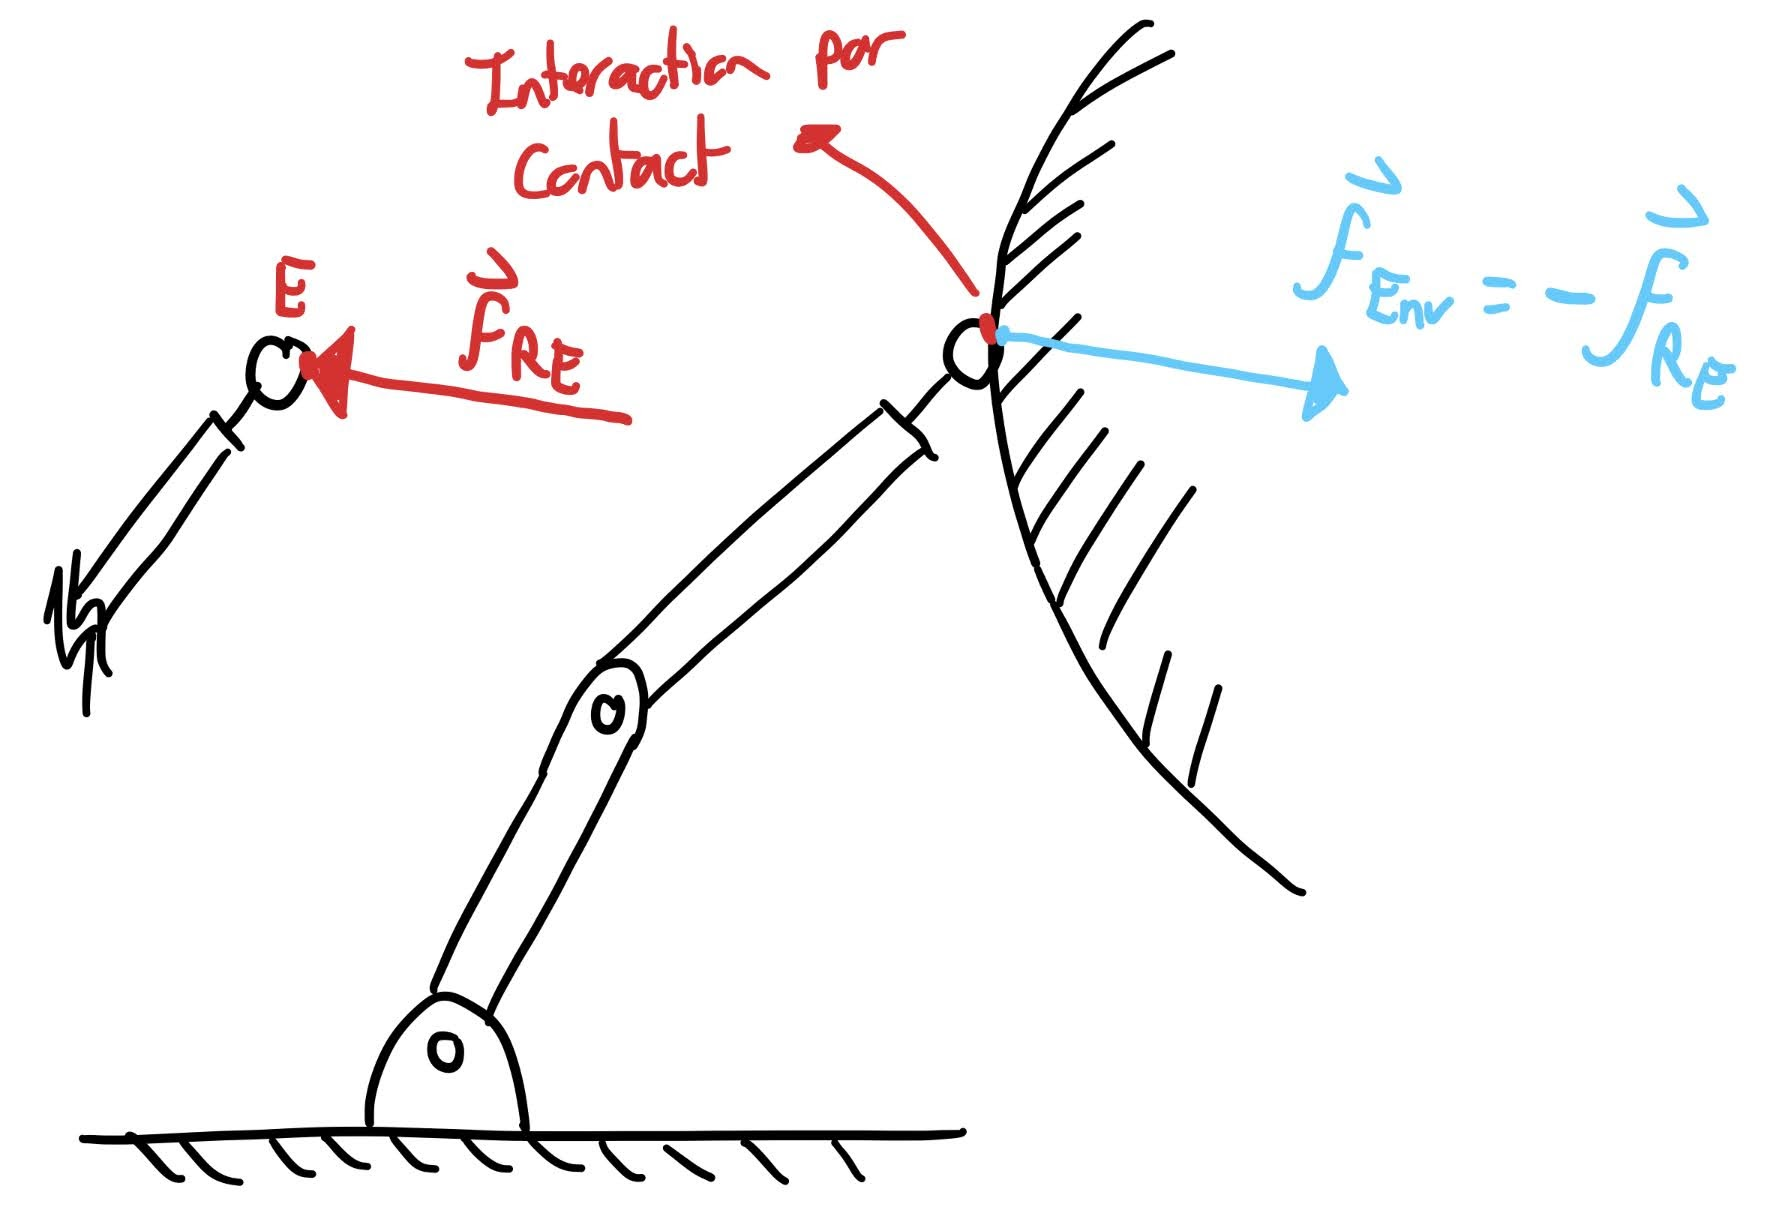
\includegraphics[width=0.65\textwidth]{fig/force_ext_contact.jpg}
	\caption{Action-réaction pour une force de contact}
	\label{fig:contactforce}
\end{figure}
%%%%%%%%%%%%%%%%%%%%%%%%%%%%%%%%

\section{Relation entre les forces aux joints et les forces à l'effecteur}
\label{sec:manipstatic}

La relation entre les forces/couples dans l'espace des joints $\col{\tau}$ et un vecteur de forces externes $\vec{f}_{R_E}$ appliquée sur l'effecteur d'un robot peut être décrite par la relation suivante:
%%%%%%%%%%%%%%%%
\begin{align}
\col{\tau} &= J\left( \, \col{q} \, \right)^T \, \col{f}_E = -J\left( \, \col{q} \, \right)^T \, \col{f}_{R_E}
\label{eq:staticmanipulator}
\end{align}
%%%%%%%%%%%%%%%
où la matrice Jacobienne $J$ est la même matrice de la relation de cinématique différentielle de l'équation \ref{eq:diffkinrel}. Comme illustré à la Figure \ref{fig:controlvolume}, les variables de forces/couples doivent correspondent aux même dégrées de liberté que les variables vitesses associées à la relation de cinématique différentielle. 




\begin{proof}
La relation statique qui implique le Jacobien (eq. \eqref{eq:staticmanipulator}) peut être déterminée à partir d'un bilan de puissance. Si on applique la 1ère loi de la thermodynamique au volume de contrôle indiqué à la Figure \ref{fig:controlvolume} pour calculer le bilan d'énergie:
%%%%%%%%%%%%%%%%
\begin{align}
\frac{dE}{dt} = P_{in} - P_{out}
\end{align}
%%%%%%%%%%%%%%%
Les forces internes inertielles et dissipatrices sont ici négligés pour trouver une relation valide dans des conditions quasi-statique. De plus considérons d'abord un cas sans force conservatrice (voir section \ref{sec:manipstaticconservative} pour ce cas) Dans ces conditions, il n'y a aucune accumulation d'énergie interne: les seules entrée/sorties de puissance dans le système sont le travail mécanique fait par les actionneurs sur le robot, et le travail mécanique fait par le robot sur l'environnement. L'égalité du travail mécanique en entrée et sortie peut être convertie en relation matricielle:
%%%%%%%%%%%%%%%%
\begin{align}
P_{in} &= P_{out} \\
\dot{q}_1 \tau_1  + \dot{q}_2 \tau_2 + \hdots  &= \Vec{v} \bullet \Vec{f}_E \\
\left[ \begin{array}{c c c} 
\dot{q}_1 & \dot{q}_2 & \hdots 
\end{array} \right] \,
\left[ \begin{array}{c} 
\tau_1 \\ \tau_2 \\ \vdots 
\end{array} \right] &= \col{\dot{r}}^T \col{f}_E \\
\col{\dot{q}}^T \col{\tau} &= \col{\dot{r}}^T \col{f}_E \\
\end{align}
%%%%%%%%%%%%%%%
Ensuite, si on substitut les composantes du vecteur vitesse de l'effecteur $\col{\dot{r}}$ par l'équation de cinématique différentielle directe (eq. \eqref{eq:diffkinrel}), on obtient:
%%%%%%%%%%%%%%%%
\begin{align}
\col{\dot{q}}^T \col{\tau} &= \left( J( \col{q}) \,  \col{\dot{q}}  \right)^T \col{f}_E \\
\col{\dot{q}}^T \col{\tau} &= \col{\dot{q}}^T  J( \col{q})^T \col{f}_E    \\
\col{\dot{q}}^T \Big( \col{\tau} \Big) &= \col{\dot{q}}^T  \Big( J( \col{q})^T \col{f}_E \Big)   
\quad \Rightarrow \quad \col{\tau} = J\left( \, \col{q} \, \right)^T \, \col{f}_E 
\end{align}
%%%%%%%%%%%%%%%
Donc les deux termes qui multiplient (produit intérieur) le vecteur colonne $\col{\dot{q}}$ doivent nécessairement être égaux, se qui nous donne l'équation qui relie les forces dans l'espace des joints aux forces équivalentes dans l'espace de la tâche. 
\end{proof}


\subsection{Flux de puissance}

Du point de vue du flux de puissance dans le système robotique, de l'énergie électrique vers le travail mécanique fait par le robot, la Jacobien peut-être vue comme une matrice de ratios de transformation. Par exemple, les Figures \ref{fig:robotpowerflow1} et \ref{fig:robotpowerflow2} illustrent quelques unes des transformations de puissance dans un système robotique et les paramètres associées. Dans chacun des domaines la puissance est caractérisée par deux variables, une de flux (courant, vitesse, débit, etc.) et une de d'effort (tension, couple, force, pression, etc.). La puissance est le produit de ces deux variables, ou le produit intérieur des vecteurs-colonnes de ces variables dans le cas de systèmes multi-variables. Le flux de puissance peut être transformé par des dispositifs qu'on appelle des transformateurs. Un transformateur amplifie la variable de flux et réduit la variable d'effort, ou vice-versa. Par exemple, les transformateurs électriques qui réduise la tension dans un réseau électrique, les transmissions mécaniques avec ratios de réduction, etc. Lorsqu'un dispositif transfert la puissance sous une forme d'énergie différente, on les appelle des transducteurs, par exemple un moteur électrique. La puissance en entrée et en sortie des transformateurs est conservée, si l'effort est amplifié d'un facteur $T$ le flux est réduit d'un facteur $T$. 

\video{Flux de puissance pour un robot manipulateur}{https://youtu.be/qyrFzkjPhHY}

%%%%%%%%%%%%%%%%%%%%%%%%%%%%%%%%
\begin{figure}[htpb]
	\centering
		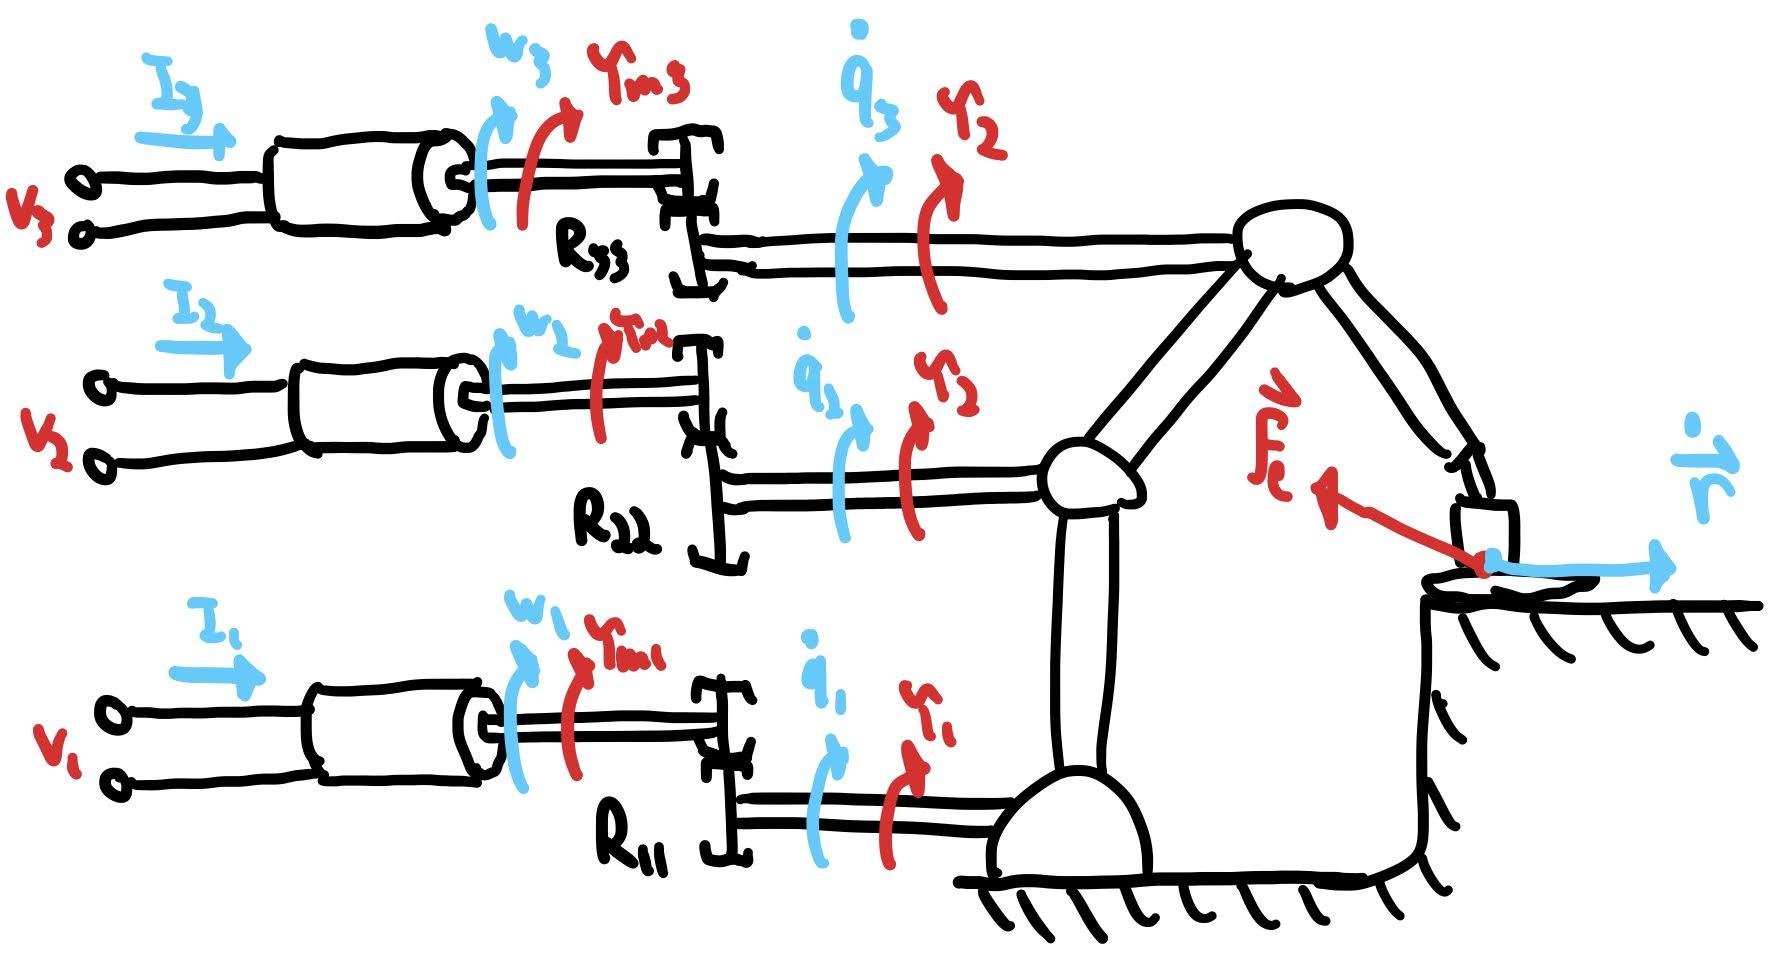
\includegraphics[width=0.60\textwidth]{fig/robotpowerflow1.jpg}
	\caption{Flux de puissance: les variables de flux et d'effort dans les différents domaines et espaces du robot.}
	\label{fig:robotpowerflow1}
\end{figure}
%%%%%%%%%%%%%%%%%%%%%%%%%%%%%%%%

Les Figures \ref{fig:robotpowerflow1} et \ref{fig:robotpowerflow2} illustrent les trois transformations de puissances principales dans un bras robotique typique. La puissance électrique est transformée en puissance mécanique des l'arbre des moteurs par les moteurs électriques, ensuite celle-ci est transformée en puissance mécanique dans les joints du robot par les transmissions, et finalement la puissance mécanique dans les joints est transformé en puissance mécanique à l'effecteur du robot. La première transformation est caractérisée par les constantes moteurs $k_m$:
%%%%%%%%%%%%%%%%
\begin{align}
%\text{\underline{Scalaire}} \quad \quad \text{Multi-DDL } \\
\tau = k_m I \\%\quad \quad  \col{\tau} &= K \col{I} \\
v = k_m w %\quad \quad  \col{v} &= K \col{w}
\end{align}
%%%%%%%%%%%%%%%
la deuxième transformation est caractérisée par les ratios de réductions des transmissions $R$:
%%%%%%%%%%%%%%%%
\begin{align}
\tau = R \tau_m \\%\quad \quad  \col{\tau} &= R \col{\tau_m } \\
w = R \dot{q} %\quad \quad  \col{w} &= R \col{q}
\end{align}
%%%%%%%%%%%%%%%
et la dernière transformation est caractérisée par la matrice Jacobienne du robot $J$:
%%%%%%%%%%%%%%%%
\begin{align}
\col{\tau} &= J^T \col{f}_E \\
\col{\dot{r}} &= J \col{\dot{q}}
\end{align}
%%%%%%%%%%%%%%%

%%%%%%%%%%%%%%%%%%%%%%%%%%%%%%%%
\begin{figure}[H]
	\centering
		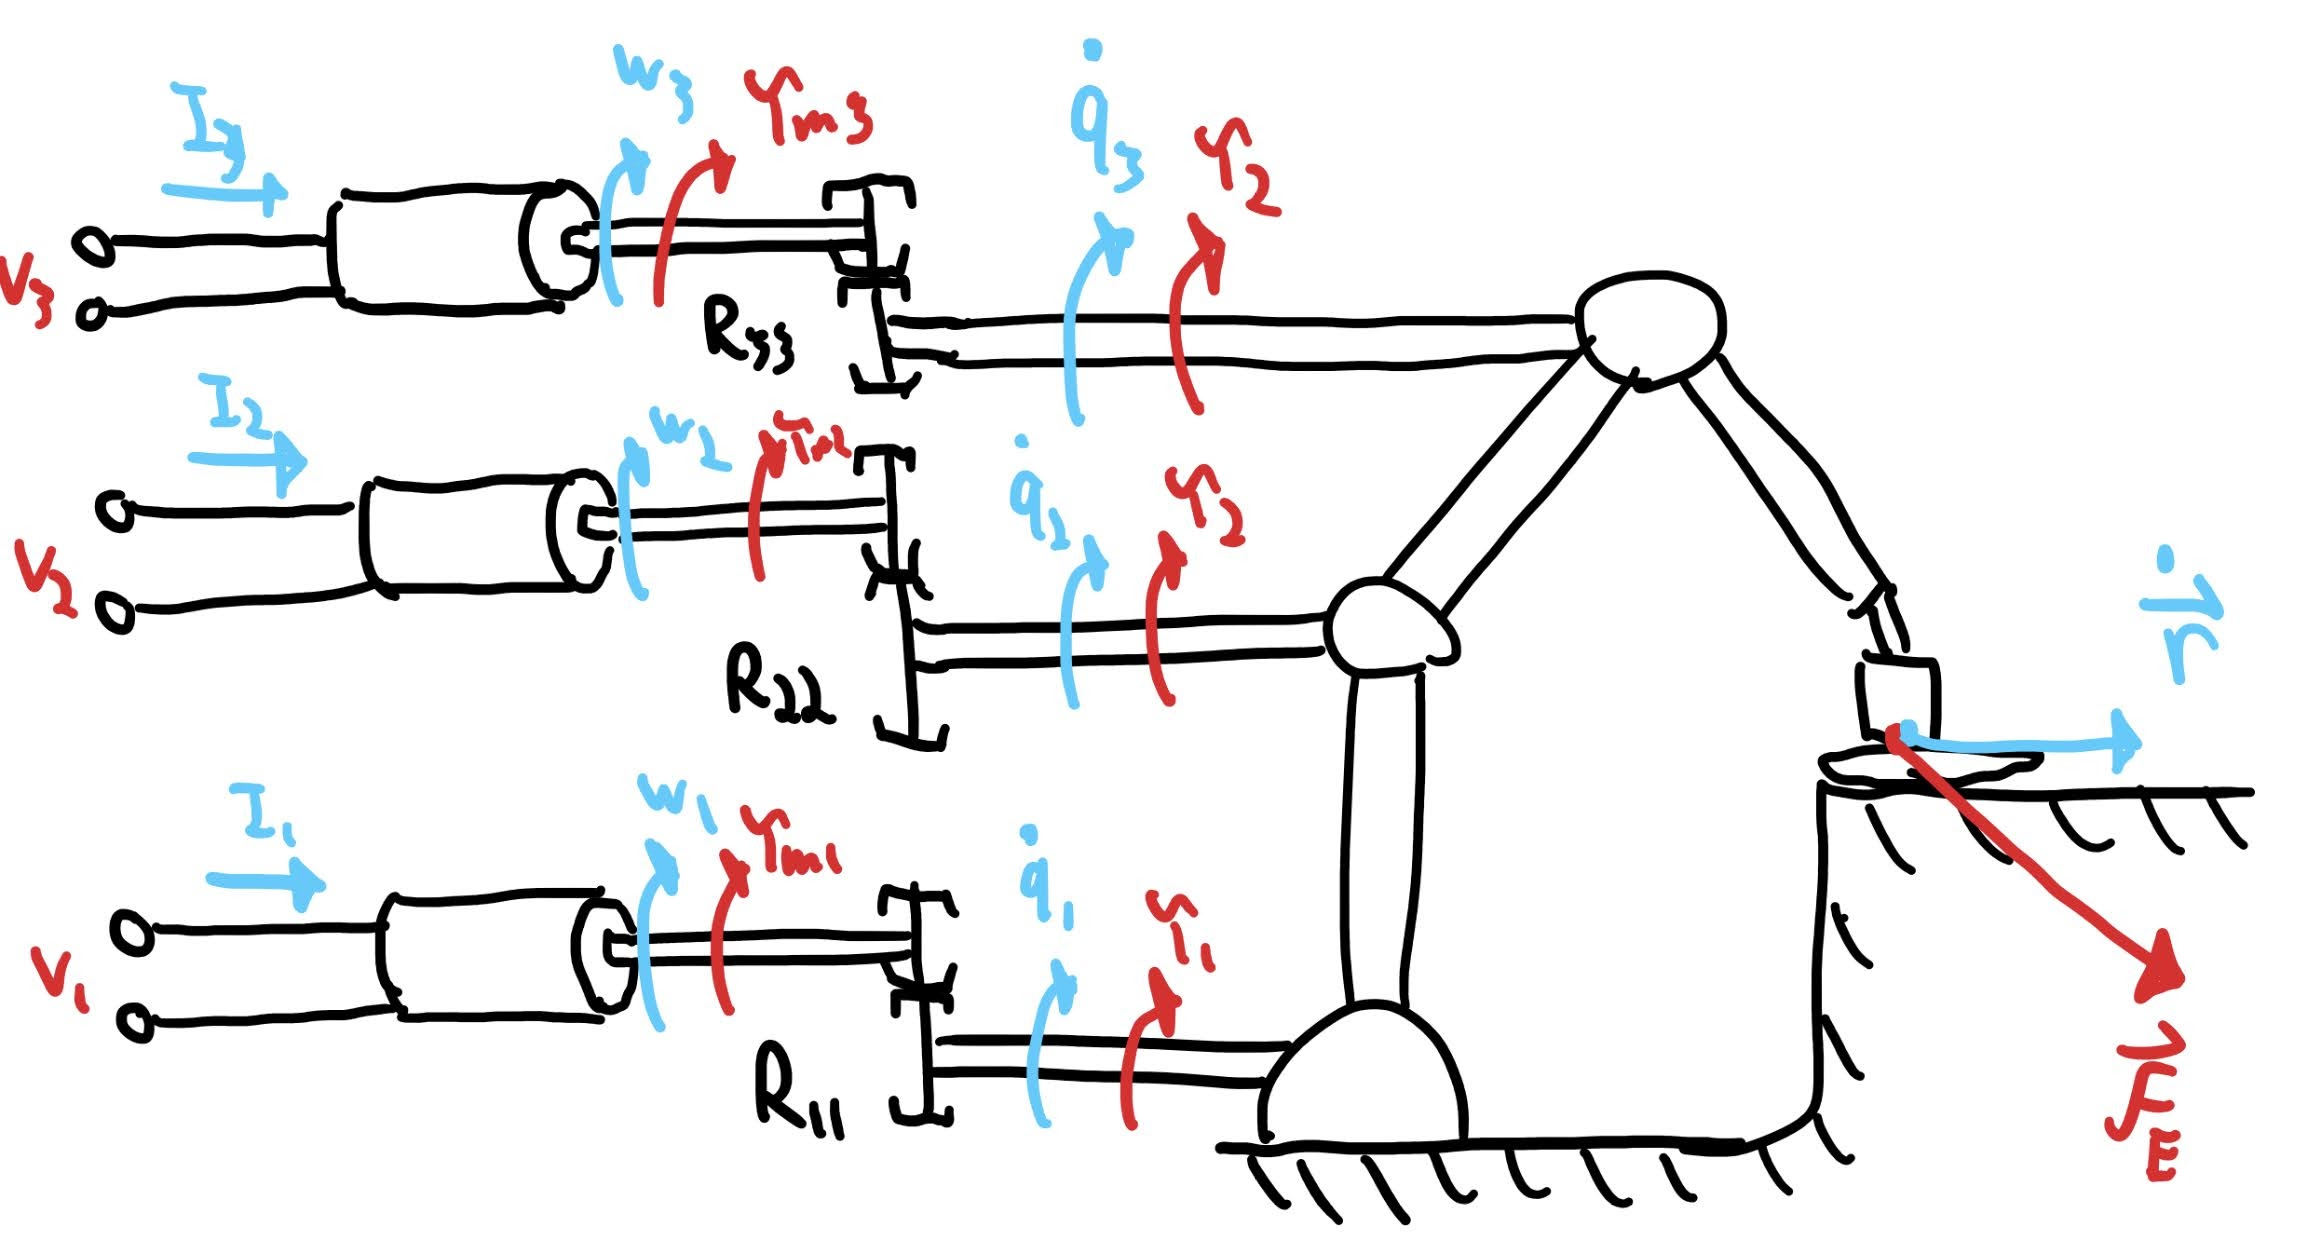
\includegraphics[width=0.70\textwidth]{fig/robotpowerflow2.jpg}
	\caption{Flux de puissance: de l'alimentation électrique vers le travail sur la charge}
	\label{fig:robotpowerflow2}
\end{figure}
%%%%%%%%%%%%%%%%%%%%%%%%%%%%%%%%





\begin{example}[Relation statique pour un robot simple à un DDL]

La Figure \ref{fig:static1dofexemple} illustre un la matrice Jacobienne d'un robot simple à 1 DDL, pour lequel l'espace de la tâche est simplement la position horizontale $x$ de l'effecteur. Pour ce système à une entrée et une sortie, la matrice Jacobienne est de dimension $1\times1$, donc un scalaire qui ici correspond à la hauteur de l'effecteur du robot. La vitesse $\dot{x}$ pour une vitesse angulaire $\dot{\theta}$ donnée est fonction de cette hauteur. Finalement, le lien entre une force horizontale à l'effecteur et le couple équivalent au joint est aussi fonction de cette même hauteur. 

%%%%%%%%%%%%%%%%%%%%%%%%%%%%%%%%
\begin{figure}[H]
	\centering
		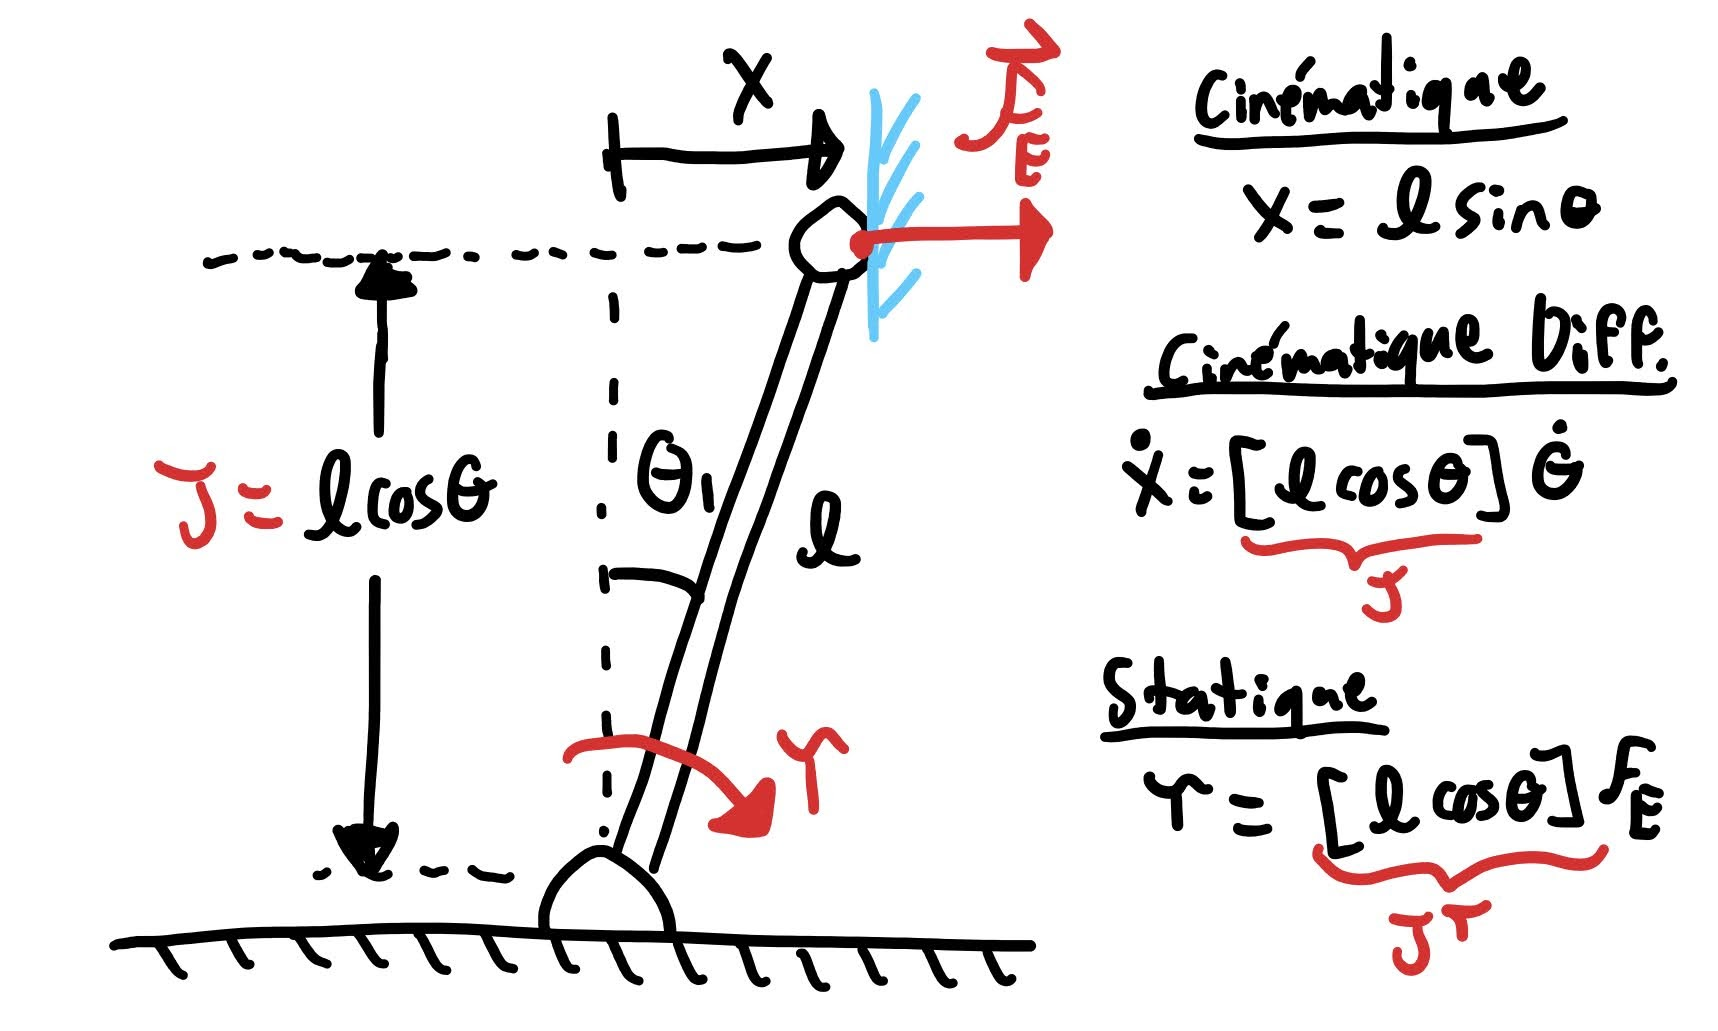
\includegraphics[width=0.70\textwidth]{fig/static1dofexemple.jpg}
	\caption{Exemple de la relation statique pour un manipulateur à 1 DDL}
	\label{fig:static1dofexemple}
\end{figure}
%%%%%%%%%%%%%%%%%%%%%%%%%%%%%%%%
\end{example}

\subsection{Relation statique sur une singularité}

Lorsqu'un robot manipulateur est sur une singularité, la transposée de la matrice Jacobienne est caractérisée par une amplification d'un facteur zéro pour certaines direction spécifique de vecteur force externe. Cela signifie que aucun couple dans l'espace des joints est nécessaire pour résister à une force externe dans cette direction. De façon générale si le un robot est proche d'une singularité, très peu de couple aux joint est nécessaire pour résister à certaines directions de forces externes. La marche humaine est particulièrement efficace car nos jambes sont maintenues dans des configurations proches de singularité qui permette de résister à la charge gravitationnelle avec peu d'effort musculaire. 
%%%%%%%%%%%%%%%%%%%%%%%%%%%%%%%%
\begin{figure}[H]
	\centering
		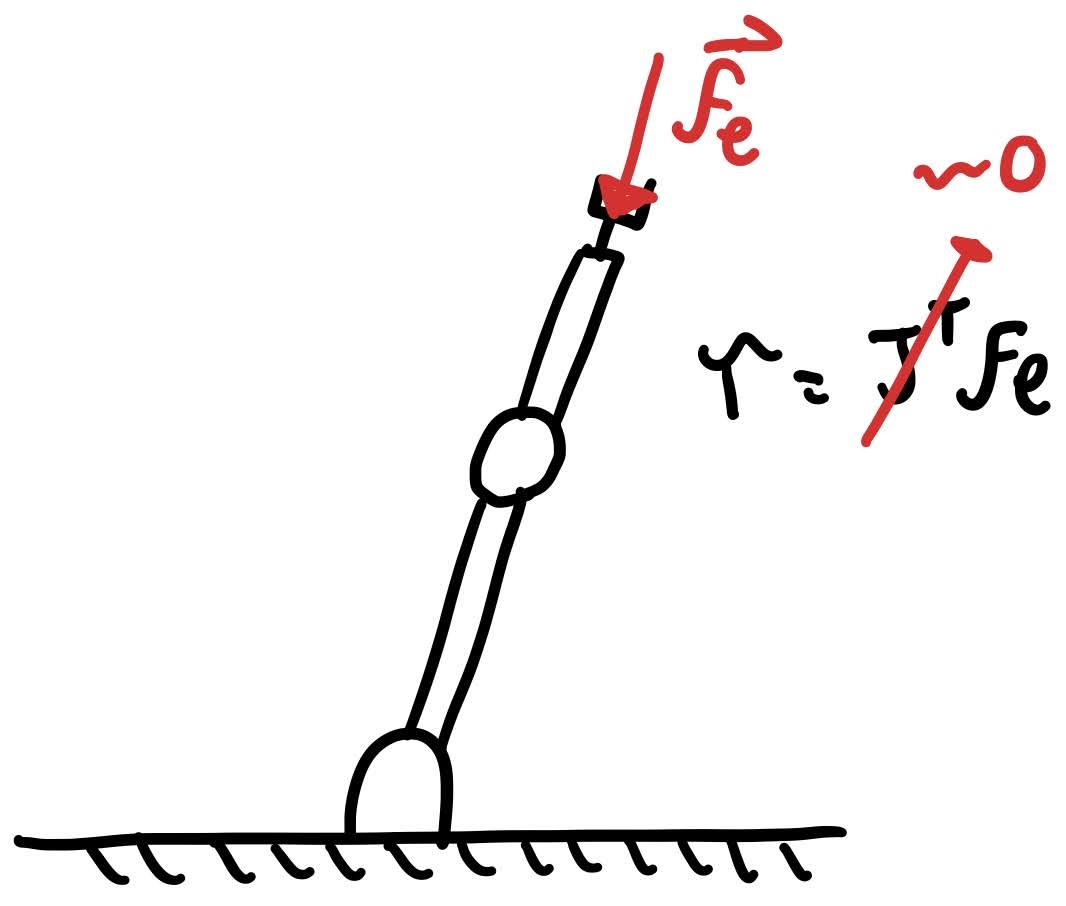
\includegraphics[width=0.45\textwidth]{fig/externalforcesingularity.jpg}
	\caption{Relation statique sur une singularité}
	\label{fig:externalforcesingularity}
\end{figure}
%%%%%%%%%%%%%%%%%%%%%%%%%%%%%%%%


\section{Relation statique incluant les forces conservatrices}
\label{sec:manipstaticconservative}

Si la bilan d'énergie effectué à la section \ref{sec:manipstatic} est fait en incluant l'énergie potentielle, un terme de forces conservatrices $\col{g}$ doit être ajouté à l'équation de la balance des forces dans le systèmes. On nommera ici ce vecteur $\col{g}$ car pour les robots manipulateur, c'est généralement un vecteur de forces gravitationnelles. 

%%%%%%%%%%%%%%%%
\begin{align}
\col{\tau} &= J\left( \, \col{q} \, \right)^T \, \col{f}_E +  g( \col{q} )
\quad \quad \text{avec:  }
\underbrace{ \col{g} ( \col{q} ) = 
\frac{ \partial V(\col{q} ) }{\partial \col{q}^T } 
}_{\text{Gradient de l'énergie potentielle}}
\label{eq:staticgravity}
\end{align}
%%%%%%%%%%%%%%%

\note{Note:}{Le vecteur colonne par lequel on prend les dérivés partielles de $V$ est ici noté avec une transposition pour respecter la convention (voir section \ref{sec:vectoropindex}) pour obtenir pour $\col{g}$ un vecteur-colonne $n \times 1$ plutôt que un vecteur-rangé $1 \times n$. }

\begin{proof}
Le nouveau terme provient du fait que la variation de l'énergie interne du système n'est pas nulle, car l'énergie potentielle du système varie selon le travail effectué par les forces conservatrices:
%%%%%%%%%%%%%%%%
\begin{align}
E = V( \col{q} ) \quad \Rightarrow \quad \frac{dE}{dt} = \frac{dV}{dt} = \frac{\partial V}{ \partial \col{q}} \, \frac{d \col{q}}{dt} = \frac{\partial V}{ \partial \col{q}} \, \col{\dot{q}}
\end{align}
%%%%%%%%%%%%%%%
On obient alors:
%%%%%%%%%%%%%%%%
\begin{align}
\frac{dE}{dt} &= P_{in} - P_{out} \\
\frac{\partial V}{ \partial \col{q}} \, \col{\dot{q}} &=  \col{\dot{q}}^T \col{\tau} - \col{\dot{q}}^T  J( \col{q})^T \col{f}_E  \\
\col{\dot{q}}^T  \, \Big(  \frac{\partial V}{ \partial \col{q}^T} \Big) &=  \col{\dot{q}}^T  \Big(\col{\tau} -  J( \col{q})^T \col{f}_E  \Big)
\end{align}
%%%%%%%%%%%%%%%
Donc pour que la relation de puissance soit respecté, les termes qui multiplie le vecteur-colonne de vitesses doivent être égaux, ce qui donne la relation entre les forces de l'équation \eqref{eq:staticgravity}.
\end{proof}


\video{Relation statique d'un robot manipulateur incluant la gravité}{https://youtu.be/RcARRDVzrm8}


\newpage
%%%%%%%%%%%%%%%%%%%%%%%%%%%%%%%%%%%%%%%%%%%%%%%%%%%%%%%%%%%%%%%%
\section{Relation de la compliance aux joints et à l'effecteur}
\label{sec:manipcompliance}

Lorsque les robots sont contrôlé en position par des servo-moteurs à chaque joint, chacun de ces moteurs et sa boucle d'asservissement en position peut être représenté comme une rigidité dans l'espace des joints, i.e. une variation du couple produit par le joint pour un déplacement de ce joint par rapport à la configuration que le contrôleur tente de maintenir:
%%%%%%%%%%%%%%%%
\begin{align}
\delta \tau_i = k_i \delta q_i \quad \Rightarrow \quad \delta \col{\tau} = K_q \, \delta \col{q}
\end{align}
%%%%%%%%%%%%%%%
où $K_q$ est une matrice de rigidité dans l'espace des joints. Il est ensuite intéressant de déterminer la rigidité d'un robot, comme illustré à la Figure \ref{fig:robotcompliance}, lorsqu'il subit une force externe en fonction de la rigidité angulaire de ses servo-moteurs.
%%%%%%%%%%%%%%%%%%%%%%%%%%%%%%%%
\begin{figure}[htbp]
	\centering
		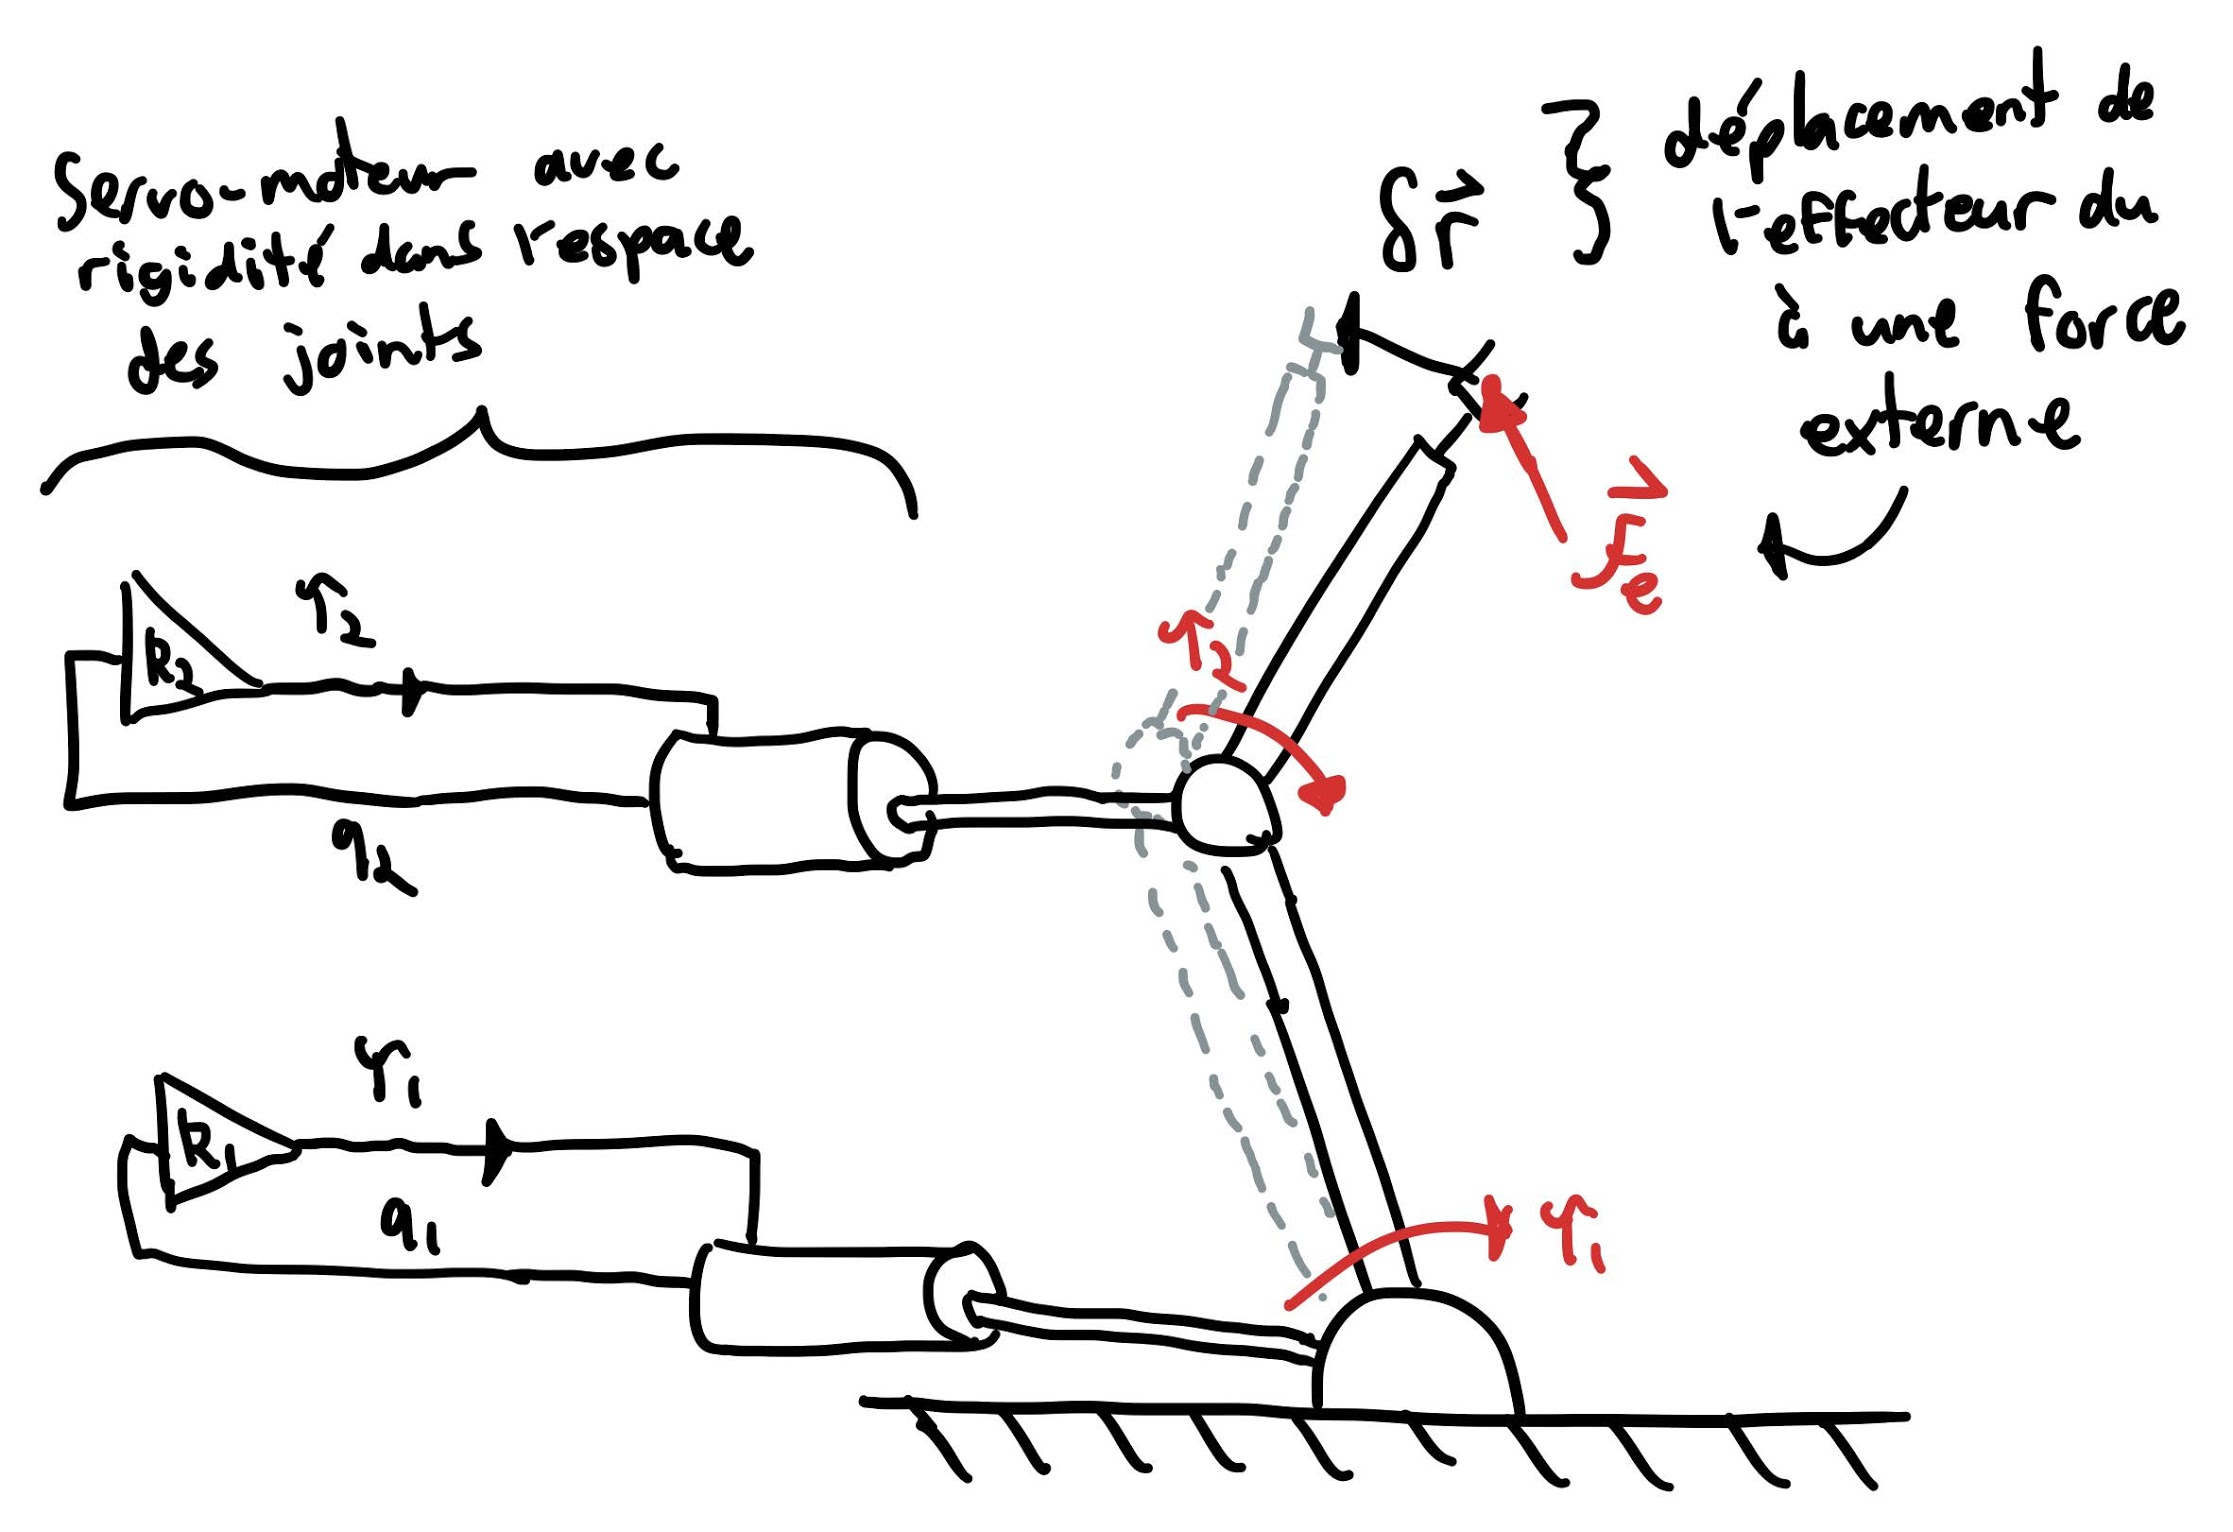
\includegraphics[width=0.70\textwidth]{fig/robotcompliance.jpg}
	\caption{Compliance d'un robot à une force externe}
	\label{fig:robotcompliance}
\end{figure}
%%%%%%%%%%%%%%%%%%%%%%%%%%%%%%%%
La variation de position de l'effecteur peut être reliée aux déplacement angulaire dans l'espace des joints, et la force externe peut être transformée en couples équivalents à chacun des joints (pour un équilibre statique). En manipulant les équations on obtient:
%%%%%%%%%%%%%%%%
\begin{align}
\delta \col{r} = J \delta \col{q} = J K_q^{-1} \col{\tau} = 
\underbrace{
\left[ J K_q^{-1} J^T \right]
}_{C_r} \,  \col{f}_{R_E}
\end{align}
%%%%%%%%%%%%%%%
où $C_r$ est une matrice de compliance à l'effecteur. La rigidité apparente à l'effecteur, due à un rigidité dans l'espace des joints, est donc donnée par une relation qui relie la variation de la position de l'effecteur à un force externe appliquée sur l'effecteur:
%%%%%%%%%%%%%%%%
\begin{align}
\col{f}_E = -\col{f}_{R_E} = - K_r \delta \col{r} \quad \text{avec } K_r = C_r^{-1} = \left[ J K_q^{-1} J^T \right]^{-1}
\end{align}
%%%%%%%%%%%%%%%
Comme illustré à la Figure \ref{fig:robotcompliance_effector}, la matrice de rigidité dans l'espace des joints est généralement diagonale (les moteurs sont indépendents). Il est à noter que la matrice de rigidité à l'effecteur est dépendante de la configuration nominale du robot (i.e. $J$ est une fonction de $\col{q}$ en général).
%%%%%%%%%%%%%%%%%%%%%%%%%%%%%%%%
\begin{figure}[htbp]
	\centering
		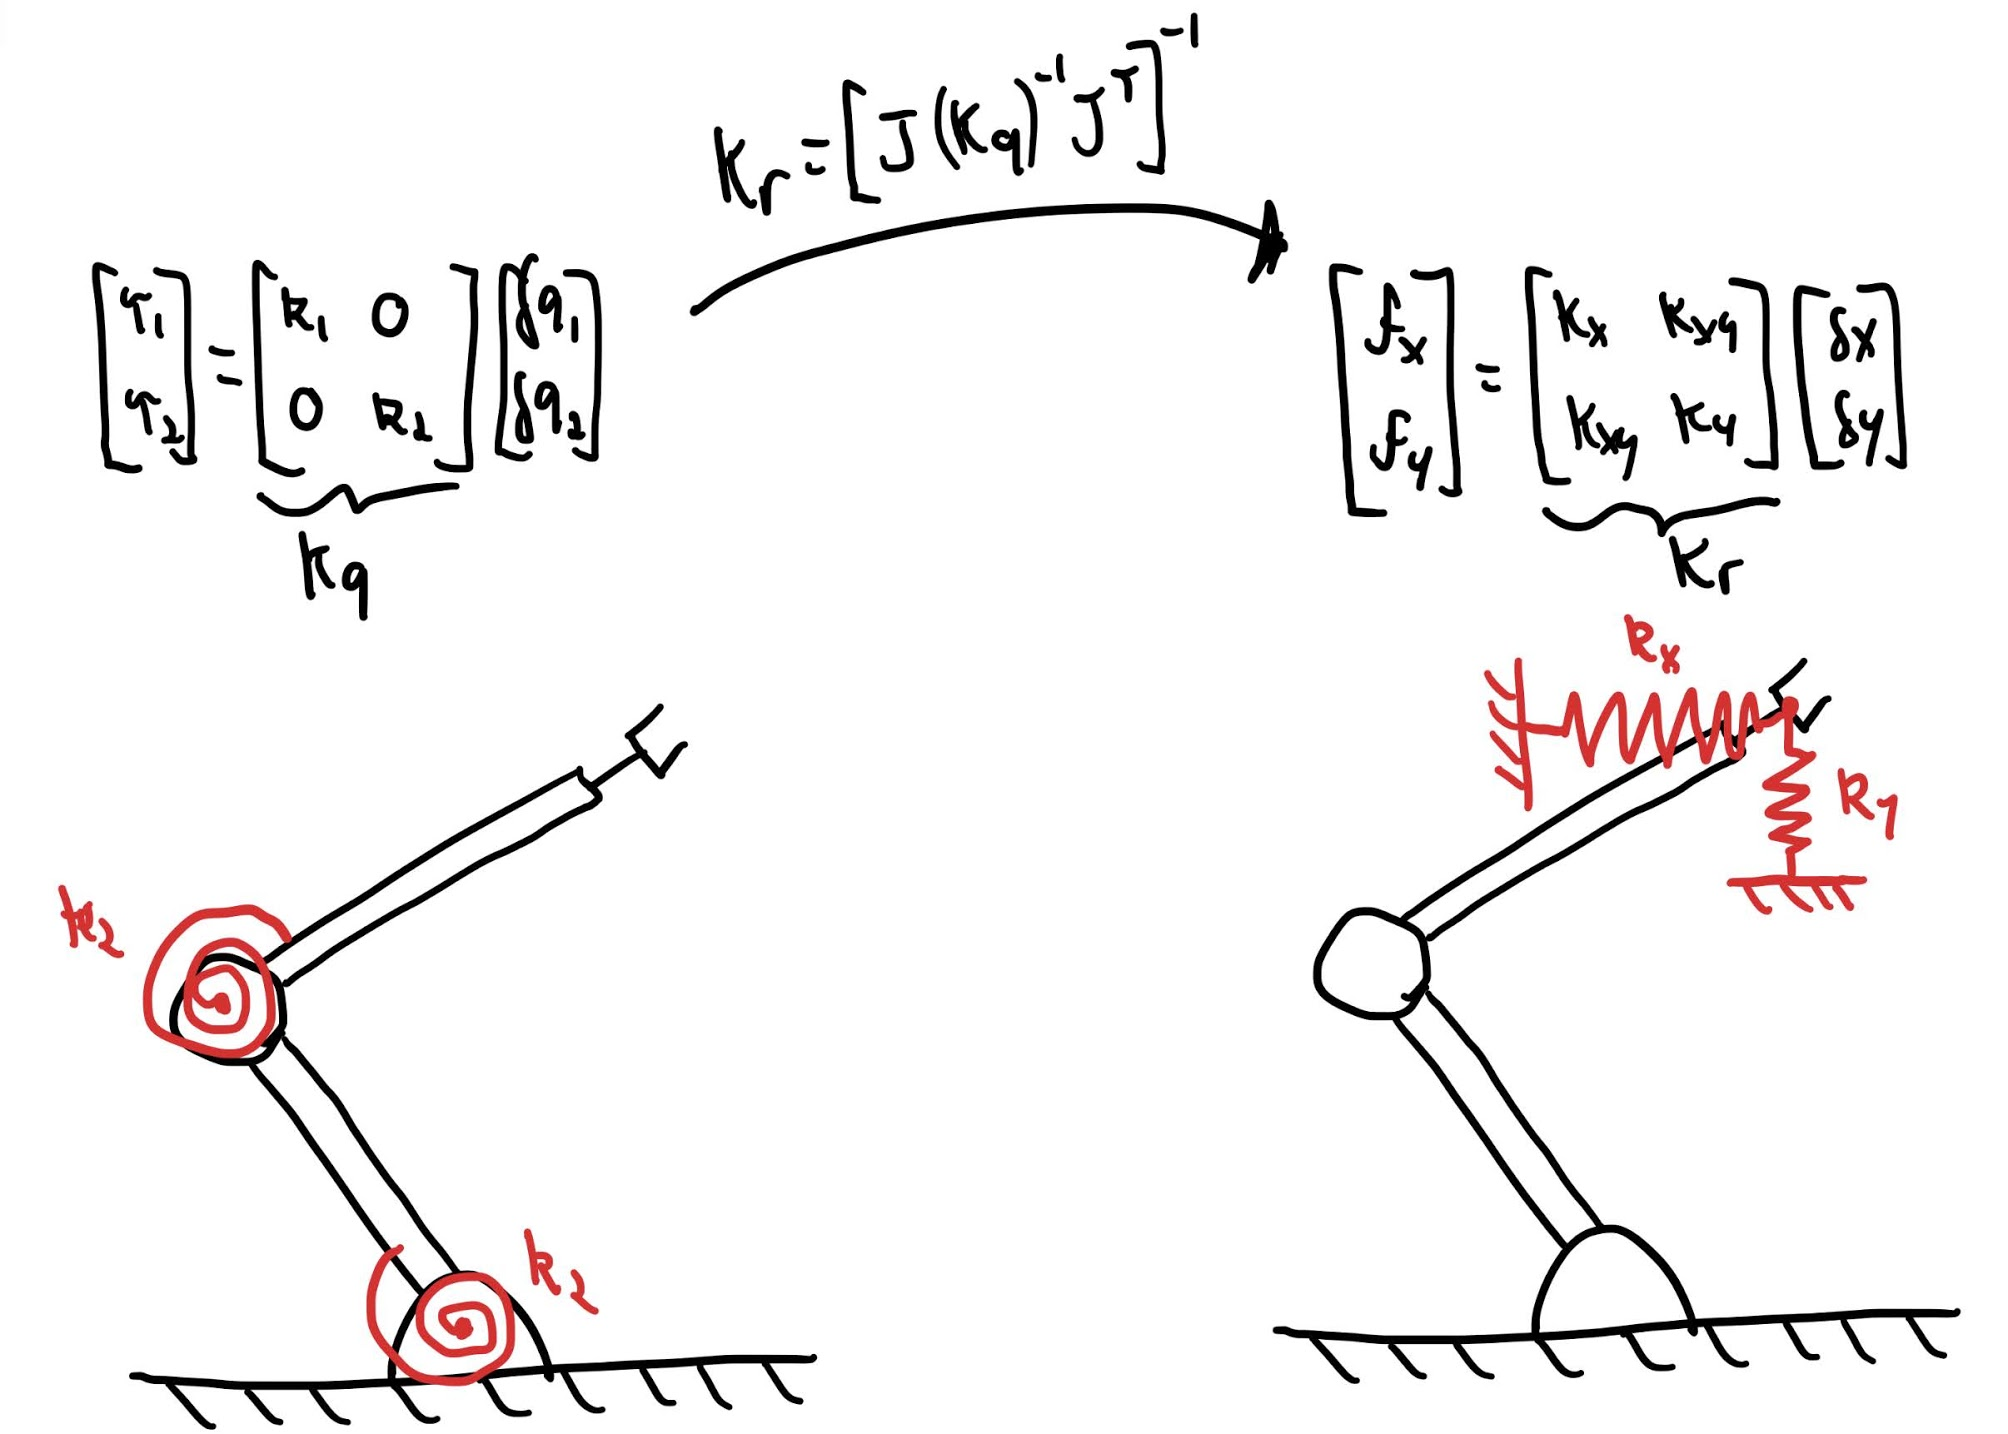
\includegraphics[width=0.80\textwidth]{fig/robotcompliance_effector.jpg}
	\caption{Matrice de rigidité équivalente d'un robot dans l'espace de l'effecteur}
	\label{fig:robotcompliance_effector}
\end{figure}
%%%%%%%%%%%%%%%%%%%%%%%%%%%%%%%%
%
Finalement, il est à noter que la matrice $C$ de compliance est singulière lorsque le Jacobien est singulier, donc sur une singularité un robot manipulateur a une ou des directions avec aucune compliance, i.e. infiniment rigide, comme illustré à la Figure \ref{fig:robotcompliance_singular}.
%%%%%%%%%%%%%%%%%%%%%%%%%%%%%%%%
\begin{figure}[htbp]
	\centering
		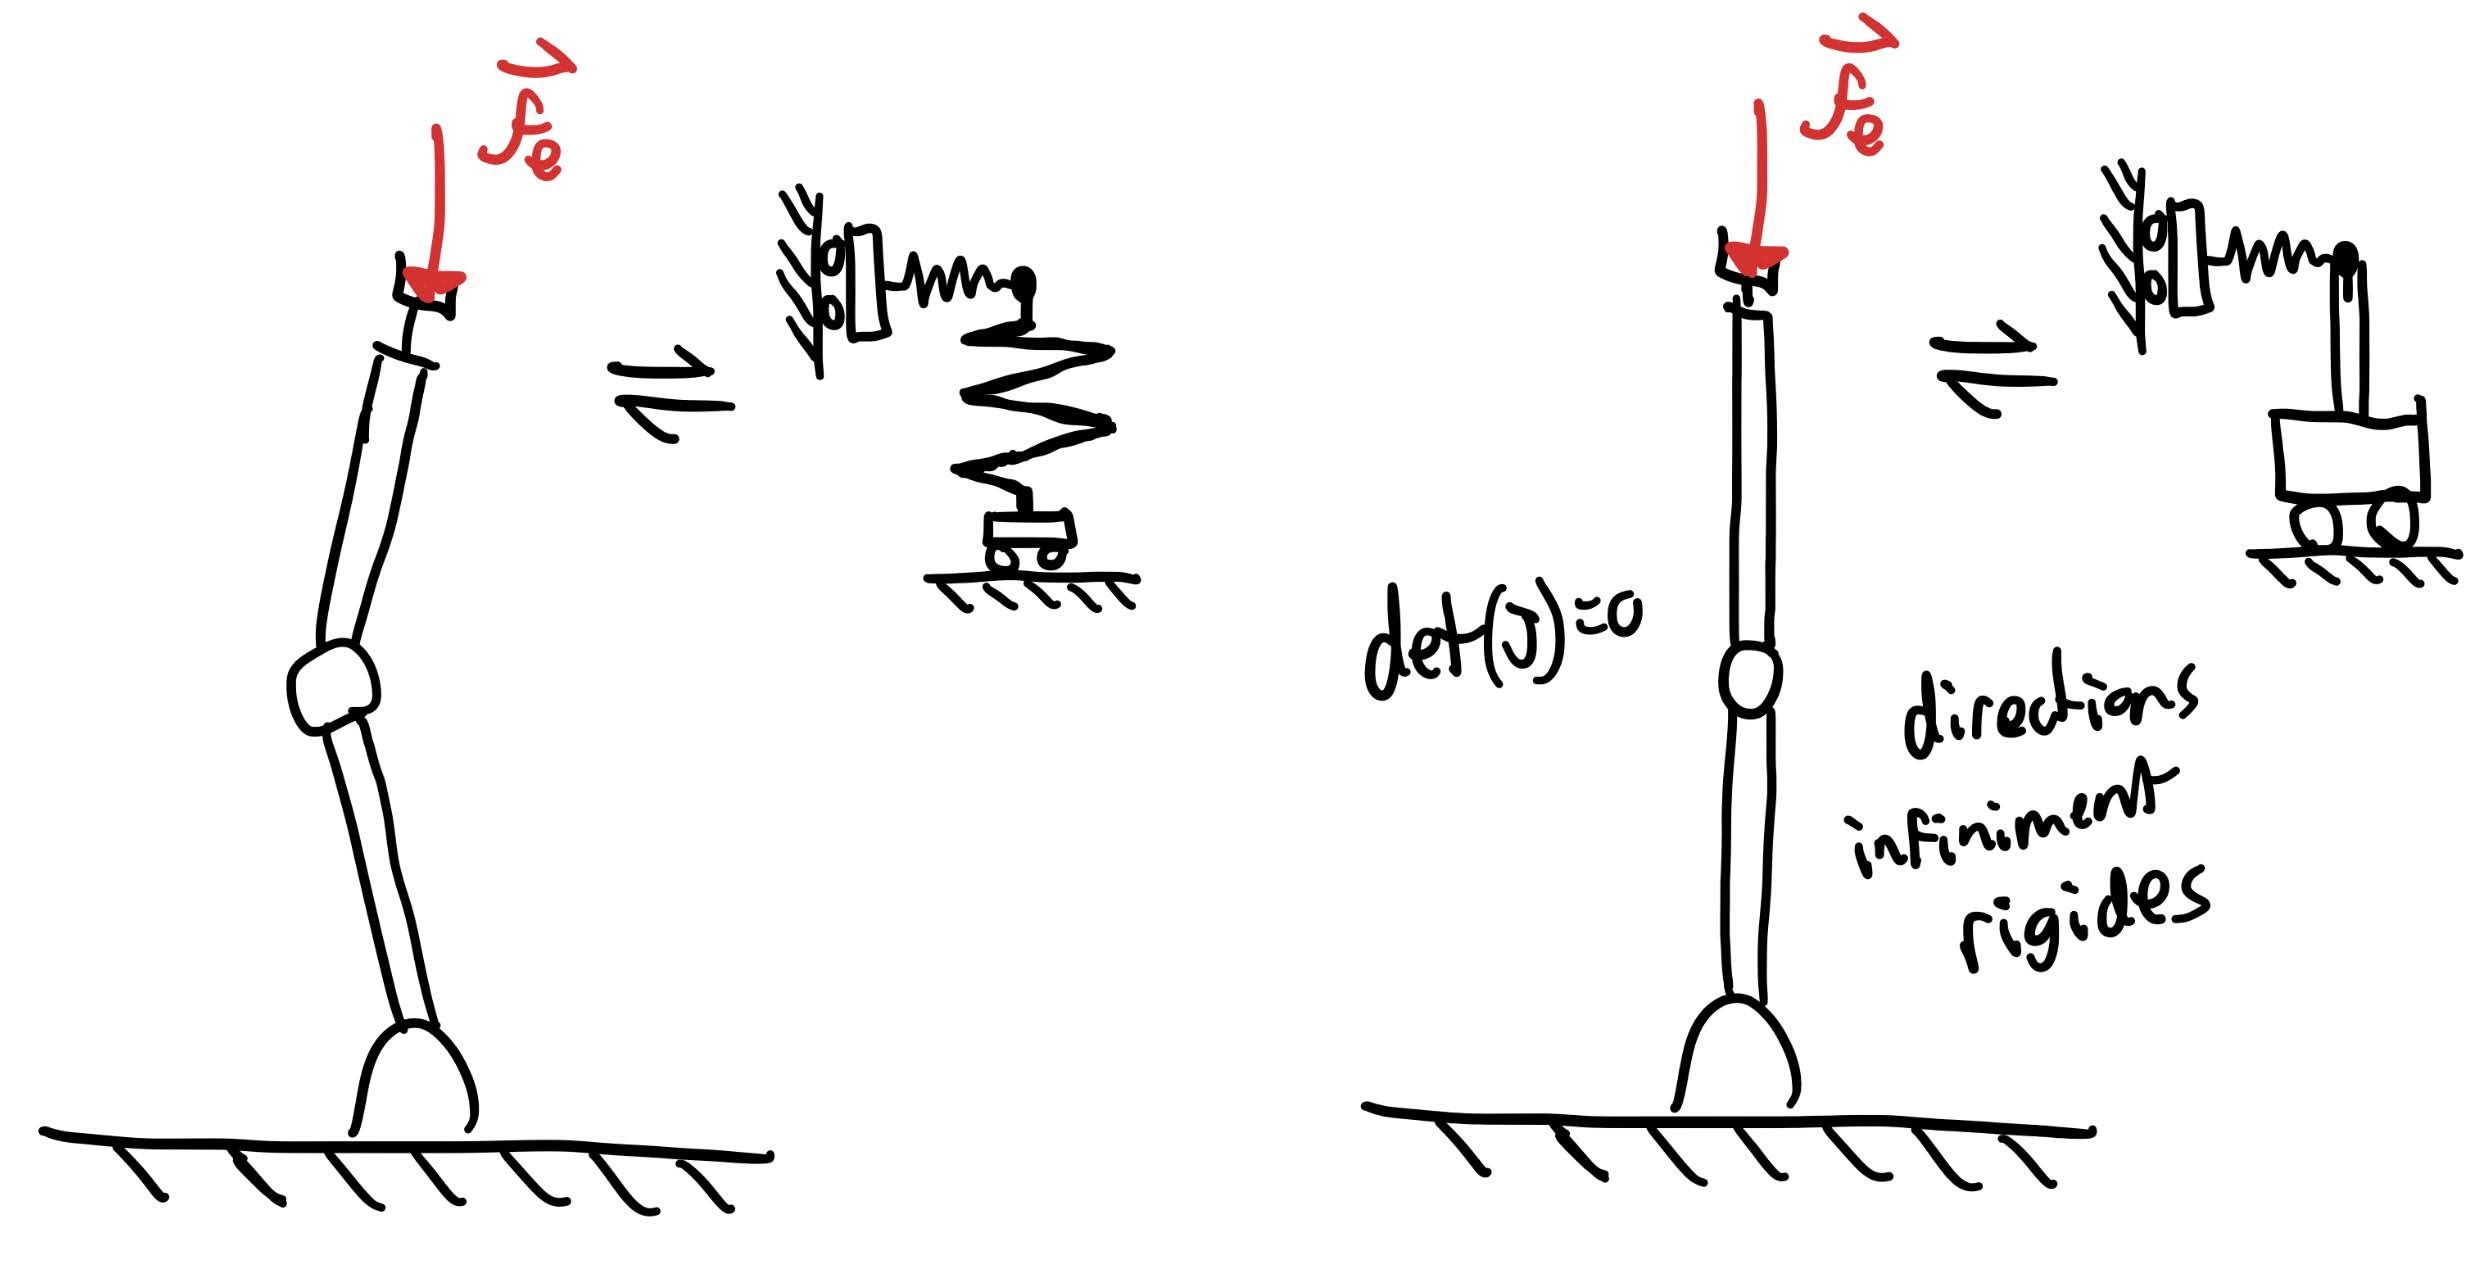
\includegraphics[width=0.80\textwidth]{fig/robotcompliance_singular.jpg}
	\caption{Effet des configuration singulière sur la rigidité d'un robot manipulateur}
	\label{fig:robotcompliance_singular}
\end{figure}
%%%%%%%%%%%%%%%%%%%%%%%%%%%%%%%%

\video{Compliance et rigidité des robots manipulateurs}{https://youtu.be/U3fhFlkVoEg}



%%%%%%%%%%%%%%%%%%%%%%%%%%%%%%%%%%%%%%%%%%%%%%%%%%%%%%%%%%%%%%%%
\newpage
\section{Manipulabilité en force d'un robot manipulateur}
\label{sec:manipforceelipse}

L'ellipsoïde de force d'un robot manipulateur est l'enveloppe des vecteurs forces possibles à l'effecteur pour des vecteurs d'entrée $\tau$ unitaires (typiquement des couples moteurs), voir \ref{fig:manipulabilityellipsoid_force}. L'enveloppe de forces possibles à l'effecteur, résultant d'un vecteur de couples des joints unitaire, peut être calculer en débutant avec une équation qui contraint la norme du vecteur de couple des joint et en substituant $\col{\tau}$ par $J^{T} \col{f}_E$ dans l'équation:
%%%%%%%%%%%%%%%%%%%%%%%%%%%%%%%%%%%
\begin{align}
1 &= \col{\tau}^T \col{\tau} \\
1 &= (J^{T} \col{f}_E)^T J^{T} \col{f}_E \\
1 &= \col{f}_E^T \, (J J^{T} ) \, \col{f}_E \\
1 &= \col{f}_E^T  \, A \, \col{f}_E \quad\quad \text{avec} \quad\quad A = J J^T
\end{align} 
%%%%%%%%%%%%%%%%%%%%%%%%%%%%%%%%%%%
On voit donc que c'est la même matrice $J J^T$ qui caractérise l'ellipsoïde de manipulabilité en force que celle qui caractérise l'ellispoïde de vitesse (voir section \ref{sec:velocitymanipulability}, mais ici c'est l'inverse de la matrice qui apparaît. Les axes principaux sont donc les mêmes mais les amplitudes sont inversés par rapport à l'ellispoïde. Par exemple, si le vecteur de vitesse possible à l'effecteur est faible dans une certaine direction, les forces externes possible à soutenir dans cette même direction vont être grandes. De plus, sur une singularité, il y a des directions pour lesquelles le vecteur vitesse possible est nul, ce qui va correspondre à des direction pour lesquelles le vecteur force possible va tendre vers l'infini, ce qui correspond à une direction pour laquelle une force externe va être reprise par la structure sans effort requis par les actionneurs.

%%%%%%%%%%%%%%%%%%%%%%%%%%%%%%%%
\begin{figure}[htbp]
	\centering
		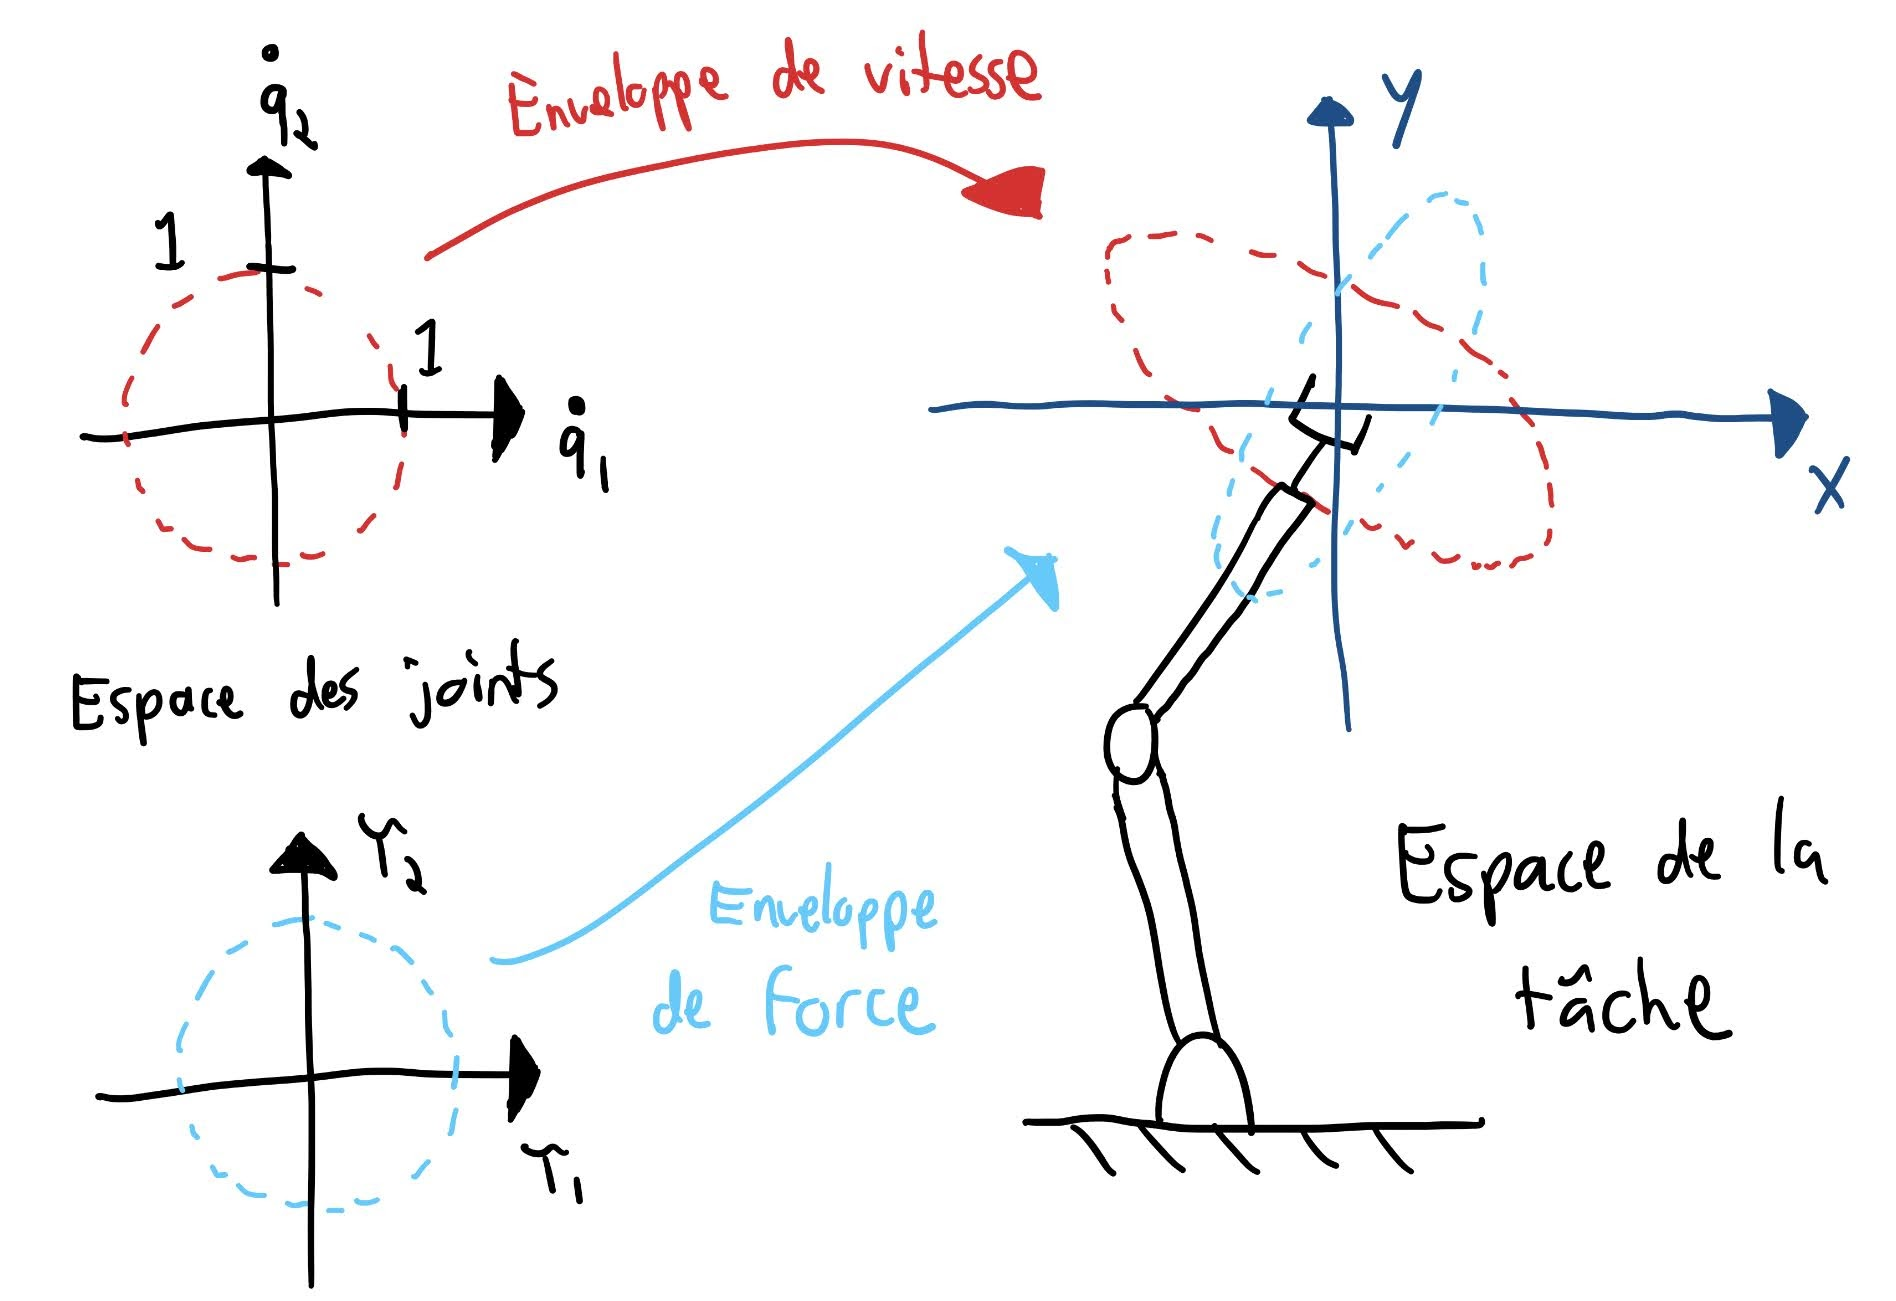
\includegraphics[width=0.90\textwidth]{fig/forcemanipulabilityellipsoid.jpg}
	\caption{Ellispoïde de manipulabilité pour la force et la vitesse}
	\label{fig:forcemanipulabilityellipsoid}
\end{figure}
%%%%%%%%%%%%%%%%%%%%%%%%%%%%%%%%



\begin{example}[Exemples d'ellispoïdes de manipulabilité pour un robot 2DDL]

La Figure \ref{fig:manipulabilityellipsoidexemples} illustre un robot 2DDL planaire dans quelques configurations. Lorsque le robot est dans une configuration avec le coude partiellement plié les capacités du robot sont le plus isotropique. Lorsque le coude est déplié le robot est capable de supporter des grande forces dans la direction radiale et l'inverse lorsque le coude est complètement plié. 
%%%%%%%%%%%%%%%%%%%%%%%%%%%%%%%%
\begin{figure}[H]
	\centering
		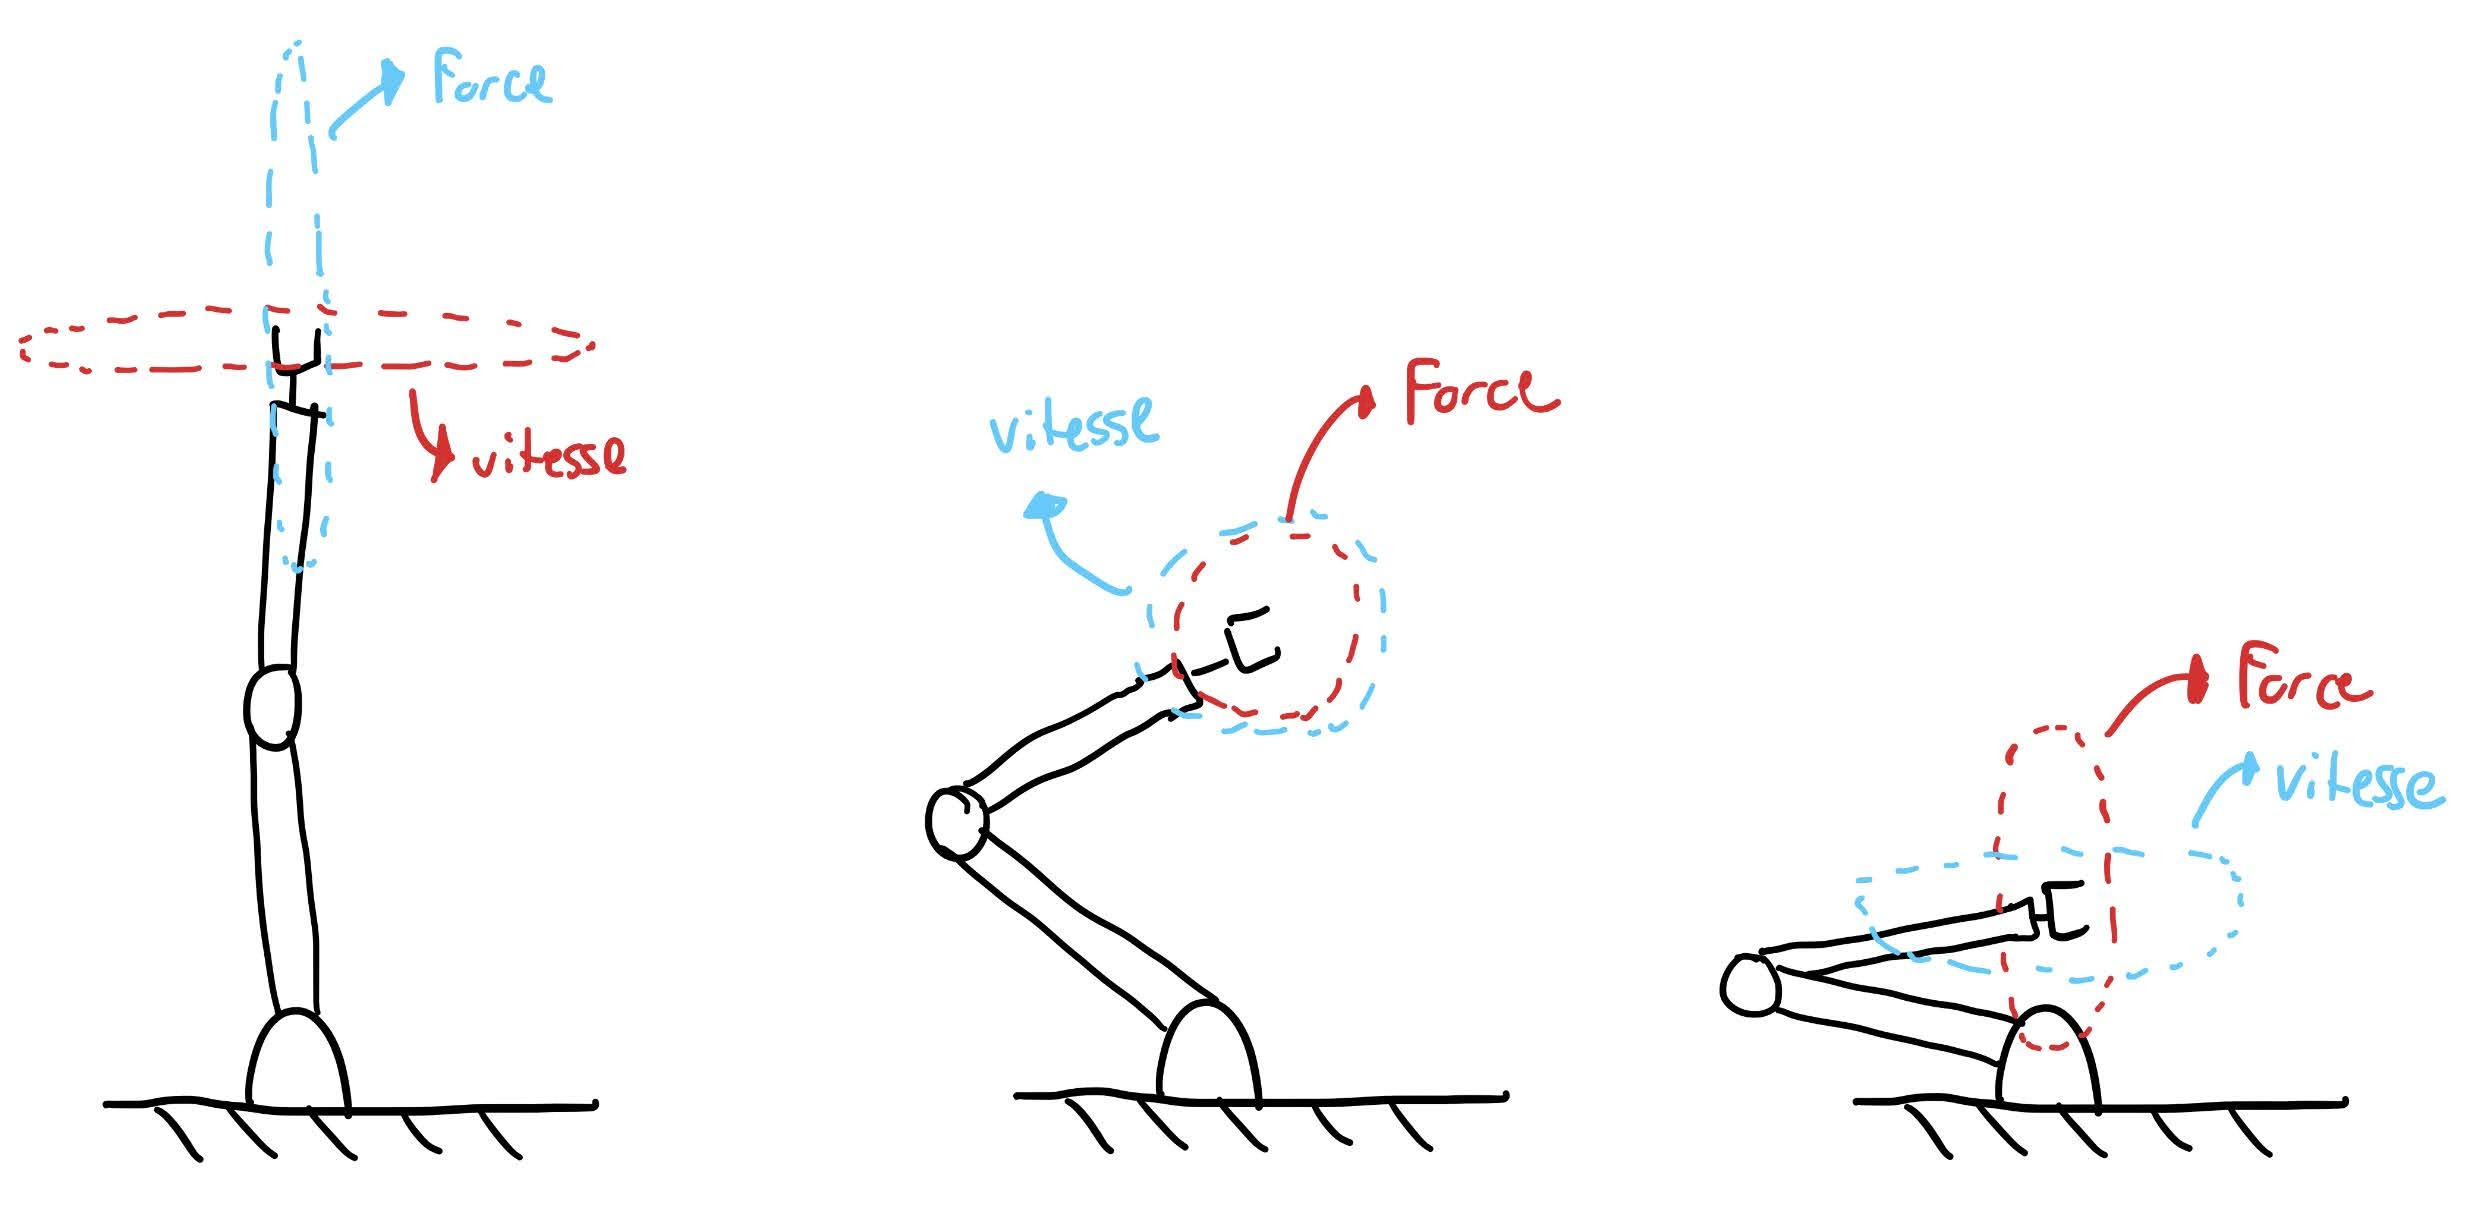
\includegraphics[width=0.95\textwidth]{fig/manipulabilityellipsoidexemples.jpg}
	\caption{Exemples d'ellispoïde de manipulabilité pour divers configration}
	\label{fig:manipulabilityellipsoidexemples}
\end{figure}
%%%%%%%%%%%%%%%%%%%%%%%%%%%%%%%%
Notre expérience humaine peut nous aider à avoir une intuition à savoir comment des propriétés peuvent être exploitées. Comme exercice de pensée je vous suggère de réfléchir à divers tâches du quotidien, la configuration de nos bras et jambe naturellement utilisé et les requis en force/vitesse: Comment configurez vous votre coude pour pousser contre une lourde porte? Quelle est la configuration naturelle de votre bras pour écrire? Comment configurez vous votre bras pour lancer une balle le plus loin possible? Est-ce qu'il serait intéressant de marcher les genous pliés?
\end{example}


%%%%%%%%%%%%%%%%%%%%%%%%%%%%%%%%%%%%%%%%%%%%%%%%%%%%%%%%%%%%%%%%
\newpage
\section{Résumé du chapitre}

Force externes à l'effecteur:
%%%%%%%%%%%%%%%%
\begin{align}
\col{f}_{R_E} &= - \col{f}_E \\
\col{f}_{R_E} &= \text{Force appliquée sur l'effecteur du robot par l'environnement} \\
\col{f}_E &= \text{Force appliquée sur l'environnement par le robot}
\end{align}
%%%%%%%%%%%%%%%

Relation force joints-effecteur:
%%%%%%%%%%%%%%%%
\begin{align}
\col{\tau} &= J\left( \, \col{q} \, \right)^T \, \col{f}_E 
\end{align}
%%%%%%%%%%%%%%%

Équilibre statique:
%%%%%%%%%%%%%%%%
\begin{align}
\col{\tau} &= J\left( \, \col{q} \, \right)^T \, \col{f}_E +  g( \col{q} )
\quad \quad \text{avec:  }
g( \col{q} ) = 
\frac{ \partial V(\col{q} ) }{\partial \col{q} } 
\end{align}
%%%%%%%%%%%%%%%

Rigidité apparente à l'effecteur:
%%%%%%%%%%%%%%%%
\begin{align}
K_r = C_r^{-1} = \left[ J K_q^{-1} J^T \right]^{-1}
\end{align}
%%%%%%%%%%%%%%%